\documentclass[a4paper,11pt]{book}
%% Language and font encodings
\usepackage[english]{babel}
\usepackage[utf8x]{inputenc}
\usepackage[T1]{fontenc}
%% Euro symbol
\usepackage{textcomp}

%% tabel rows
%% color rows table
\usepackage{xcolor}
\usepackage{color}
\usepackage{colortbl}
\definecolor{grayrow}{rgb}{0.85, 0.85, 0.85}
\definecolor{darkgrayrow}{rgb}{0.7, 0.7, 0.7}
\definecolor{RoyalRed}{rgb}{0.61,0.11,0.19}

\usepackage{emptypage} % remove header in blanck pages

%% Sets page size and margins
\usepackage[a4paper,top=3cm,bottom=2cm,left=3cm,right=3cm,marginparwidth=1.75cm]{geometry}

%% Useful packages
\usepackage{amsmath}
\usepackage{graphicx}
\usepackage{epigraph}
%\usepackage[colorinlistoftodos]{todonotes}
\usepackage[colorlinks=true, allcolors=blue]{hyperref}

% include file and not recompile it
\usepackage{standalone}
\usepackage{dsfont}

%% images directory
\graphicspath{{img/}}
%% colors
\hypersetup{
colorlinks,
citecolor=black,
filecolor=black,
linkcolor=black,
urlcolor=blue
}

\usepackage{numprint}
\npthousandsep{\,}

\usepackage{listings}

\definecolor{codegreen}{rgb}{0,0.6,0}
\definecolor{codegray}{rgb}{0.5,0.5,0.5}
\definecolor{codepurple}{rgb}{0.58,0,0.82}
\definecolor{backcolour}{rgb}{0.95,0.95,0.92}

\lstdefinestyle{snippet}{
    backgroundcolor=\color{backcolour},
    commentstyle=\color{codegreen},
    keywordstyle=\color{magenta},
    numberstyle=\tiny\color{codegray},
    stringstyle=\color{codepurple},
    basicstyle=\ttfamily\footnotesize,
    breakatwhitespace=false,
    breaklines=true,
    captionpos=t,
    keepspaces=true,
    numbers=left,
    numbersep=5pt,
    showspaces=false,
    showstringspaces=false,
    showtabs=false,
    tabsize=2
}

\lstdefinestyle{c++}{
    backgroundcolor=\color{backcolour},
    commentstyle=\color{green}\ttfamily,
    keywordstyle=\color{blue}\ttfamily,
    numberstyle=\tiny\color{codegray},
    stringstyle=\color{red}\ttfamily,
    basicstyle=\ttfamily\footnotesize,
    morecomment=[l][\color{magenta}]{\#}
    breakatwhitespace=false,
    breaklines=true,
    captionpos=t,
    keepspaces=true,
    numbers=left,
    numbersep=5pt,
    showspaces=false,
    showstringspaces=false,
    showtabs=false,
    tabsize=2
}

\lstdefinestyle{Java}{
    backgroundcolor=\color{backcolour},
    commentstyle=\color{green}\ttfamily,
    keywordstyle=\color{blue}\ttfamily,
    numberstyle=\tiny\color{codegray},
    stringstyle=\color{red}\ttfamily,
    basicstyle=\ttfamily\footnotesize,
    showspaces=false,
    showtabs=false,
    breaklines=true,
    showstringspaces=false,
    breakatwhitespace=true,
    commentstyle=\color{codegray},
    keywordstyle=\color{blue},
    stringstyle=\color{red},
    basicstyle=\ttfamily,
    moredelim=[il][\textcolor{codegray}]{$$},
    moredelim=[is][\textcolor{codegray}]{\%\%}{\%\%}
}

\usepackage[]{algorithm2e}

%% Custom commands

\newcommand{\quotes}[1]{``#1''}

%% Start Document
\begin{document}

\documentclass{standalone}

\begin{document}

\begin{titlepage}

%\centering
%\includegraphics[scale=0.5]{unibo.png}

\begin{center}
{{\Large{\textsc{Alma Mater Studiorum $\cdot$ Universit\`a di Bologna}}}}
\rule[0.1cm]{15.8cm}{0.1mm}
\rule[0.5cm]{15.8cm}{0.6mm}
\\\vspace{3mm}

{\small{\bf Dottorato di Ricerca in Fisica\\Ciclo 32}}

\end{center}

{\small{\bf Settore Concursuale: 02/D1}}


{\small{\bf Settore Scientifico Disciplinare: FIS/07}}

\vspace{23mm}

\begin{center}\textcolor{black}{
{\Large{\bf Implementation and optimization of algorithms\\in Biomedical Big Data Analytics}}\\
}\end{center}

\vspace{70mm} \par \noindent

\begin{minipage}[t]{\textwidth}
{\large{\bf Supervisore: \vspace{2mm}\\\textcolor{black}{
Prof. Daniel Remondini}}}\\\\
{\large{\bf Co-Supervisori: \vspace{2mm}\\\textcolor{black}{
Prof. Gastone Castellani\\
Prof. Armando Bazzani}}}\\\\
\end{minipage}


\hfill

\begin{minipage}[t]{\textwidth}\raggedleft \textcolor{black}{
{\large{\bf Presentata da:
\vspace{2mm}\\
Nico Curti}}\\
{\large{\bf Coordinatore Dottorato:
\vspace{2mm}\\
Prof.ssa Silvia Arcelli
}}}
\end{minipage}

\vspace{17mm}

\begin{center}
{\large{\bf Esame finale anno \textcolor{black}{2020}
}}
\end{center}

\end{titlepage}

\end{document}

\thispagestyle{empty}

\begin{flushright}
%% insert inscription (page 2)
\end{flushright}

%% Epigraph
\chapter*{}
\pagenumbering{gobble}% Remove page numbers (and reset to 1)
\epigraph{\quotes{\emph{No one know nothing,\\everyone know something,\\but something is nothing to someone,\\while\\something is important to everybody}}}{Daudi, Manyara}
%\epigraph{\quotes{\emph{Software is like sex:\\it's better when it's free}}{Linus Torvalds}}

%% Abstract
\pagenumbering{gobble}% Remove page numbers (and reset to 1)
\documentclass{standalone}

\begin{document}

\chapter*{Abstract}

\end{document}


\tableofcontents
\newpage

%% Introduction

\pagenumbering{arabic}% Arabic page numbers (and reset to 1)
\documentclass{standalone}

\begin{document}

\chapter*{Introduction}\label{Introduction}\addcontentsline{toc}{chapter}{Introduction}
\markboth{Introduction}{Introduction}


% take something from the EuroPar18 introduction

% in questo lavoro si affronteranno diverse tematiche relative alla Big Data Analytics e si propongono soluzioni inerenti ad ognuna di esse con esempi sviluppati ed applicati a dati reali.
% Partendo dalla curse of dimensionality e la feature extraction (dnet), passando per la visualizzazione dei dati con le NN fino alla eterogeneità dei dati (chimera)

% definire feature come variable e dire che nel resto del testo verranno usati in maniera indistinta i due termini

\end{document}


%% Chapter 1 - DNetPRO algorithm

\documentclass{standalone}

\begin{document}

\documentclass{standalone}

\begin{document}

\chapter[Feature Selection]{Feature Selection - DNetPRO algorithm}\label{chapter1:featsel}

%Introduction to feature selection problem and theoretical background.

%Focus on biological Big Data and problems related.

After the end of the Human Genome Project (HGP, 2003)~\cite{McKinney2012} there were growing interest on biological data and their analysis.
At the same time, the availability of this type of data increased exponentially with the technological improvement of data extractors (High-Throughput technologies)~\cite{Reuter2015} and the lower production costs.
These are the main factors that allow us to go into the new scientific era of Big Data.
Biological Big Data works with very large and complex datasets which are typically impossible to store, handle and analyze using standard computers and techniques~\cite{Kumari2014}.
Just think that we need around 140~GB for the storage of the DNA of a single person and an Array Express, a compendium of public gene expression data, has more than 1.3 million of genomes which have been collected in more than \numprint{45000} experiments~\cite{Greene2014}.
Since the number of available data is getting greater, we need to design several storage databases to organize, classify and, moreover, extract information from them.
The Bioinformatics European Institute (EBI) at Hinxton (UK), which is part of the European Laboratory of Biological Molecular and one of the biggest repositories of biological data, stores 20 petabytes of genomic data and proteomics back-ups.
The amount of the genomics data is only 2 petabytes, and it doubles every year: it is not worth to remark that these quantities represent about a tenth of data stored by CERN of Ginevra~\cite{Marx2013}.
In contrary, the ability of processing data and the computational techniques of analysis do not grow in the same way.
Therefore, the gap between the growth of available data and our ability to work with them is getting bigger.

From a computational point-of-view, the Bioinformatics new-science is looking for new methods to analyze these large amount of data.
Common Machine Learning methods, i.e computational algorithms able to find significant patterns into large quantities of data, need to be optimized and modified to increase their computational and statistical performances.
To improve the computational time, we need to extend existing methods and algorithms, and to develop new dimensionality reduction techniques.
In Machine Learning, in fact, as the dimensionality of the data increases, the amount of data required to perform a reliable analysis grows exponentially\footnote{
  High dimensional data tends to become very sparse and as result it is hard to perform robust statistical evaluation on it.
  This phenomena is commonly called \quotes{curse of dimensionality}~\cite{bellman1961adaptive}.
}.
Dimensionality reduction techniques are methods able to find the more significant variables of a given problem or a combination of them, where \quotes{significant} means that these few variables (or features) preserve the information about the problem as much as possible.
High-dimensional omics data (e.g. transcriptomics through microarray or NGS, epigenomics, SNP profiling, proteomics and metabolomics, but also metagenomics of gut microbiota) pose enormous challenges on how to extract useful information from them.
One of the prominent problems is to extract low-dimensional sets of variables –~signatures~– for classification and diagnostic purposes, or to better stratify patients for personalized intervention strategies based on their molecular profile~\cite{Scotlandi2009, Chan2011, Johnson2017, Beckmann2016ReconcilingEM}.


\begin{figure}[htbp]
\centering
\def\svgwidth{0.4\textwidth}
\input{./img/distributions.pdf_tex}
\qquad\qquad
\def\svgwidth{0.4\textwidth}
\input{./img/expression.pdf_tex}
\caption{(\textbf{a}) An example in which single-parameter classification fails in predicting higher-dimension classification performance.
Both parameters (\emph{feature1} and \emph{feature2}) badly classify in 1-D, but they have a very good performance in 2D.
Moreover, classification can be easily interpreted in terms of relative higher/lower expression of both probes.
(\textbf{b}) Activity of a biological feature (e.g. a gene) as a function of its expression level:
top) monotonically increasing, often also discretized to an on/off state;
center, bottom) \quotes{windowed} behavior, in which there are two or more activity states that do not depend monotonically on expression level.
X axis: expression level, Y axis, biological state (arbitrary scales).
}
\label{fig:example}
\end{figure}

Many approaches are used to face such problems~\cite{Guyon2002}, as Elastic Net~\cite{Hughey2015}, Support Vector Machine, K-nearest Neighbor, Neural Network and Random Forest~\cite{Pang2012}.
Some methods select variables using single-variable scoring methods~\cite{Eckhard2012, Hocking1976} (e.g. Student's t test for a two-class comparison), while others search for projections in lower-dimensional variable spaces, but all these approaches could fail even in simple 2-dimensional situations (Fig.~\ref{fig:example}).
As shown in Fig.~\ref{fig:example}~(a), both variables perform poorly taken singularly, but their performance becomes optimal taking them together (in terms of linear separation of the two classes).

It is known that complex separation surfaces characterize classification tasks associated to image and speech recognition, for which Deep Networks are used successfully in recent times, but in many cases biological data, such as gene or protein expression, are more likely characterized by an up/down-regulation behavior (as shown in Fig.~\ref{fig:example}~(b) top), while more complex behaviors (e.g. a \quotes{windowed} optimal range of activity, Fig.~\ref{fig:example}~(b) bottom) are much less likely.
Discriminant-based methods (and logistic regression methods alike) can very likely provide good classification performances in these cases, if applied in at least two-dimensional spaces.
The \quotes{linearity} of these methods (that generate very simple class separation surfaces, i.e. linear or quadratic) also ensures that a \quotes{buildup} of a signature based on lower-dimensional signatures can be done.

These considerations are relevant in particular for microarray data, where we face on few samples compared to a huge amount of variables (gene probes).
This kind of problem, often called \quotes{large $N$, small $S$} problem (where $N$ is the number of features, i.e variables, and $S$ is the number of samples), tends to be prone to overfitting\footnote{
  A solution to a problem is classified as \quotes{overfitted} if small fluctuations on the data variance produces classification errors.
  This problem arises when the model perfectly fits a small training set, but it is not able to generalize to a large amount of test samples (generalization).
} and they are classified to ill-posed.
The difficulty on the features extraction can also increase due to noisy variables that can drastically affect the machine learning algorithm.
It is often difficult to discriminate between noisy and significant variables, even more as the number of variables increases.

In this thesis we propose a new method of feature selection - DNetPRO, \emph{Discriminant Analysis with Network PROcessing} - developed to outperform the problems mentioned above.
Our method is designed to gene-expression data analysis and it was tested against the most common feature selection techniques.
The method was already applied on gene-expression datasets, but my work focused on its benchmarking and optimization for Big Data applications.
The pipeline is composed by several steps and only a part of them were designed for biological application: this allows us to apply (part of) the same method also on different topics with good results (see Appendix for further information about the analyses on non-biological data).


\end{document}
 % Introduction to feature selection problem and theoretical background. Focus on biological Big Data and problems related.

\documentclass{standalone}

\begin{document}

\section[DNetPRO algorithm]{DNetPRO algorithm}\label{dnetpro:DNetPRO}

The \textsf{DNetPRO} algorithm produces multivariate signatures starting from all the couples of variables analyzed by a Discriminant Analysis.
For this reason, it can be classified as a combinatorial method and the computational time for the exploration of variable space is proportional to the square of the number of underlying variables (ranging from $10^3$ to $10^5$ in a typical high-throughput omics study).
This behavior allows to overcome some of the limits of single-feature selection methods and it provides a hard-thresholding approach compared to projection-based variable selection methods.
The combinatorial evaluation is the most time-expensive step of the algorithm and it needs an accurate algorithmic implementation for Big Data applications (see the next section for further information about the algorithm implementation strategy).
A summary of the algorithm is shown in~\ref{code:DNetPRO}.

\begin{algorithm}[H]
  \KwData{Data matrix (N, S)}
  \KwResult{List of putative signatures}
  Divide the data into training and test by an Hold-Out method\;
  \For{$couple$ $\leftarrow$ ($feature\_1$, $feature\_2$) $\in$ $Couples$}{
    Leave-One-Out cross validation\;
    Score estimation using a Classifier\;
  }
  Sorting of the couples in ascending order according to their score\;
  Threshold over the couples score ($K$best couples)\;
  \For{$component$ $\in$ $connected\_components$}{
    \eIf{$reduction$}{
      Iteratively pendant node remotion\;
    }
    Signature evaluation using a Classifier\;
  }
  \caption{DNetPRO algorithm for Feature Selection.}
  \label{code:DNetPRO}
\end{algorithm}

So, given an initial dataset, with $S$ \emph{samples} (e.g. cells or patients) each one described by $N$ observations (our \emph{variables}, e.g. gene or protein expression profiles), the signature identification can be summarized with the following steps:

\begin{itemize}

\item separation of available data into a training and test sets (e.g. 33/66, or 20/80);

\item estimation of the classification performance on the training set of all $S(S-1)/2$ variable couples through a computationally fast and reproducible cross-validation procedure (leave-one-out cross validation was chosen);

\item selection of top-performing couples through a hard-thresholding procedure.
The performance of each couple constitutes a \emph{weighted link} of a network, where the nodes are the variables connected at least through one link;

\item every \emph{connected component} which composes the network identifies a putative signature.

\item (optional) in order to reduce the size of an identified signature, the pendant nodes of the network (i.e. nodes with degree equal to one) can be removed, in a single step or recursively up to the core network (i.e. a network with all nodes with at least two links).

\item all signatures are evaluated onto the test set to estimate their performances.

\item a further cross validation step is performed (with a further dataset splitting into test and validation sets) to identify the best performing signature.

\end{itemize}

We would stress that this method is completely independent to the choose of the classification algorithm, but, from a biological point-of-view, a simple one is preferable to keep an easy interpretability of the results.
The geometrical simplicity of the resulting class-separation surfaces, in fact, allows an easier interpretation of the results, as compared to very powerful but black-box methods like nonlinear-kernel SVM or Neural Networks.
These are the reasons which lead us to use very simple classifier methods in our biological applications as diag-quadratic Discriminant Analysis or Quadratic Discriminant Analysis (Appendix A for more information about the mathematical background and their respectively implementations).
Both these methods allow fast computation and an easy interpretation of the results.
A linear separation might not be common in some classification problems (e.g. image classification), but it is very likely in biological systems, where many responses to perturbation consist in an increase or decrease of variable values (e.g. expression of genes or proteins, see Fig.~\ref{fig:example}~(b)).
This assumption is very plausible for biological data, since genes are in general up- or down-regulated in order to modify their activity and protein and metabolites most of the times respond consequently.

A second direct gain by the couples evaluation is related to the network structure: the \textsf{DNetPRO} network signatures allow a hierarchical ranking of features according to their centrality compared to other methods.
The underlying network structure of the signature could suggests further methods to improve its dimensionality reduction based on network topological properties to fit real application needs, and it could help to evaluate the cooperation of variables for the class identification.

In the end, we remark that our signatures have a purely statistical relevance by being generated with a purpose of maximal classification performance, but sometimes the selected features (e.g. genes, DNA loci, metabolites) can be of clinical and biological interest, helping to improve knowledge on the mechanism associated to the studied phenomenon~\cite{PMrna, Scotlandi2009, PMgene, Terragna}.

\end{document}
 % Method description
\documentclass{standalone}

\begin{document}

\section[Toy Model]{Synthetic dataset benchmark}\label{dnetpro:toy}

Standard feature selection algorithms evaluate the single-variable performances.
Starting from the ranked variables according to their score, a signature is obtained selecting the top scorer ones according to an hard thresholding or by an iteratively add of variables until a desired output score is reached.
This method is called $K$-best algorithm and it allows to filter the number of variables without any constrain on their mutual interaction or correlation.
On the other hand, the proposed DNetPRO algorithm tries to extract the more statistically significant variables considering the interaction between them, i.e the combination of variable-pairs.
Thus, while the $K$-best algorithm scaled according to the number of variables, the DNetPRO algorithm is more computational expensive and its used can be justify only if its efficiency can be proofed.

We developed a toy model simulation to compare the performances of the standard $K$-best algorithm with the DNetPRO one, considering either the number of samples either the number of variables.
Since the DNetPRO algorithm was designed to gene expression dataset applications our toy model should consider a large number of variables with only a relative small number of samples.
To simulate a so like synthetic dataset we used the toy model generator provided by the \href{https://scikit-learn.org/stable/modules/generated/sklearn.datasets.make_classification.html}{scikit-learn package}.
This model generator allows to set a precise number of classes and distinguish between \emph{informative features}, i.e. features which easily separate the class populations, and \emph{redundant features}, i.e. features which represent noise in our problem.
The number of informative features should be realistically small compared to the noise, so in our simulations we chose to introduce a maximum of 1\% informative features in each simulation.

We randomly generated data from Gaussian distributions with an increasing number of samples and variables, i.e dimensions.
In each simulation we split the number of samples in training and test sets (Hold-Out method, with 2/3 of data as training and 1/3 as test) and we applied the DNetPRO algorithm.
From each simulation the extracted signatures were tested against the test set and the best performing one was kept.
On the same data we applied the $K$-best algorithm and we kept the same number of variables of the DNetPRO best signature, i.e $K$ equal to the number of nodes in the DNetPRO best signature.
In this way we can compare the performances obtained on the test set by the two methods.
We would highlight that in general there is not a stop criteria on the $K$-best algorithm, so the number of variables selected could be smaller or greater than the number of DNetPRO signature nodes.
However we can reasonably assume that according to the $K$-best interpretation the selected features should be the most performing ones and adding more variables should introduce only small quantity of noise.
This justify the use of the same number of variables between the two algorithms using the DNetPRO signature as reference.
In Fig.~\ref{fig:dnetpro_toy} we show the results obtained in our simulations: the results are obtained keeping fixed the number of variables/samples and varying the number of samples/variables, Fig.~\ref{fig:dnetpro_toy}(a) and Fig.~\ref{fig:dnetpro_toy}(b) respectively.

\begin{figure}[htbp]
\centering
\def\svgwidth{0.4\textwidth}
\input{./img/samples_toy.pdf_tex}
\qquad\qquad
\centering
\def\svgwidth{0.4\textwidth}
\input{./img/features_toy.pdf_tex}
\caption{Synthetic dataset simulation.
Comparison of accuracy performances obtained by the DNetPRO algorithm and the $K$-best algorithm.
\textbf{(a - left)} Performances obtained in function of the number of samples, keeping fixed the number of variables.
\textbf{(b - right)} Performances obtained in function of the number of variables, keeping fixed the number of samples.
}
\label{fig:dnetpro_toy}
\end{figure}

For the same number of variables (Fig.~\ref{fig:dnetpro_toy}(a)) we can noticed as the two methods performs quite similarly but the DNetPRO is able to reach better performances as the number of samples increase.

This trend can be explained also in statistical terms: with small samples the variability of our (random) data is large and thus the performance distributions is more unstable.
With a greater number of samples the variances of our classes is reduced and also the statistical quantities involved in the computation of the discriminant curve can be evaluated with more accuracy.
As the number of samples increase the statistically evaluation of the variables becomes easier and increase the correspondence between the top scorer variables and the true-informative ones.
In low sample cases the quantity of noise is bigger and in an high dimensional space is harder to find the most informative directions and also noise variables could reach performances higher than informative ones.


Despite the simplicity of our toy model the DNetPRO is able to highlight its efficiency in terms of performances against the single-feature method.

A slight different behavior is shown varying the number of variables and keeping fixed the number of samples (Fig.~\ref{fig:dnetpro_toy}(b)).
In this case we have a median accuracy (black line in the plot) always higher for the DNetPRO algorithm.
With a small number of variables (left part of the plot) the $K$-best algorithm performances are more stable and only from a statistical point-of-view we can justify the efficiency of the DNetPRO algorithm (the median of the distribution is still higher compared to the $K$-best one).
As the number of variables increase also the efficiency of the DNetPRO algorithm increase until it exceeds the $K$-best algorithm (and its distribution is narrowed).
We reached this situation quite faster in our simulation since we constrained our toy model with a forced unbalance between number of samples and variables, i.e the so-called ill-posed problems.
The DNetPRO was designed to work in this situations and it is able to reach high accuracy results also in critical ill-posed problems.
The evaluation of pair of variables could be helpful to find good variables which are penalized in the single score ranking but which can demonstrate a good performance-interaction with other variables.
In this cases the DNetPRO results could be helpful also to understand the variable interactions due to the network structure of the signature that can bring to deeper considerations on the fine grain interaction of the variables in a real problem context.

This kind of toy model is considered a standard for feature extraction algorithm testing but it puts several disadvantages for the DNetPRO evaluation.
We started our discussion about the DNetPRO taking into account the two distributions of data shew in Fig.~\ref{fig:example}(a).
The DNetPRO algorithm was designed to face on that kind of situations in the better way.
The limits of our algorithm are so bounded to the sample distributions: if the informative variables are totally independent one from each other the couples evaluation does not guaranteed the best approach to the problem.
An informative variable could work better with noise data than with another informative one: in this way we could expect a star-network signature in which the central node would be the informative variable connected to a series of noise variables.
Considering the signatures extracted by the DNetPRO algorithm we noticed this kind of behavior: the core of our signatures was principally composed by informative variables (which were manually introduced so easily traced).

We have to face on also the problem of multiple putative (disjointed) signatures: the DNetPRO algorithm takes into account only the connected component with the highest score as putative signature.
If the informative variables are disjointed the corresponding star-networks will be disjointed until a common noise-variable creates a bridge between the two connected components.
This means that we have to enlarge the quantity of nodes in our signature and thus increase the difficulty in the filtering of noise.

We evaluated both these situations in our toy model simulations.
In the first case we introduced only two informative variables obtained by a sampling of the distribution shew in Fig.~\ref{fig:example}(a).
In all our simulations the DNetPRO algorithm was able to identify the couple of these variables as best putative signature.
At the same time the $K$-best algorithm find with more difficulty those variables, especially when the number of variables become greater.
Considering the distribution of single-variable scores, in fact, we could noticed as the informative variables, despite they are manually introduced, were not always the top scoring ones: in large dimensional spaces also noise-variables produced high(er) performances.

Using the same sample distributions for informative features, we manually introduced multiple couples in our dataset.
As expected the DNetPRO algorithm is not able to identify in a single connected components, and thus a single putative signature, the full set of informative variables, while the $K$-best algorithm easily find them in the top scoring ranking.
To guarantee the full set of informative features into the DNetPRO signature we had to enlarge the number of nodes and thus we had to introduce multiple noise-variables.
This highlights the limits of the DNetPRO algorithm and also the need of a (optional) filter procedure to apply to the putative signatures for these critical cases\footnote{
  In the algorithm description we discussed about the possibility of removing pendant nodes as optional filter procedure.
  In the case described above this step can help but not completely solve the problems: if there are two disjointed signatures we have to enlarge the number of nodes until we create a connection between them but this connection would be probably due to a noise variable.
  The pendant nodes remotion can help to reduce the amount of node but the link which connects the two components would be preserved.
}.

%Method description.
%Efficiency on a biological toy model.

\end{document} % efficiency on a biological toy model

\documentclass{standalone}


\begin{document}

\section[DNetPRO Implementation]{Algorithm implementation}\label{implementation:implementation}

The \textsf{DNetPRO} algorithm is made by a sequence of different steps which have to be performed sequentially for a signature extraction.
For this purpose, each step can be optimized independently by using the full set of available computational resources\footnote{
Further optimization can be performed in a cross validation environment and they will be discussed later in this section.
}.
In this section it will be analyzed each part of the pipeline focusing on the optimization strategies used for the algorithm implementation.

The full code is open source and available at~\cite{DNetPRO}.
The code installation is automatically tested using \href{https://github.com/Nico-Curti/DNetPRO/blob/master/.travis.yml
}{\textsf{travis}} (for Linux and MacOS environments) and \href{https://github.com/Nico-Curti/DNetPRO/blob/master/appveyor.yml}{\textsf{appveyor}} (for Windows environments) at every commit.
The installation can be performed using \href{https://github.com/Nico-Curti/DNetPRO/blob/master/CMakeLists.txt}{\textsf{CMake}} and a full set of installation instructions can be found in the on-line project documentation.

The \textsf{Python} version of the algorithm (see next sections) can be installed via \href{https://github.com/Nico-Curti/DNetPRO/blob/master/setup.py}{\textsf{setup.py}} and the compilable parts of it checked via \textsf{CMake}.
The \textsf{Python} installer provides also the full list of dependencies of the project, which will be automatically installed by the main.

In the Github repository, it can be found also a full list of example scripts and utilities to obtain the results showed in the next sections.
We provide also the complete benchmark pipeline used in our simulation and able to run on cluster environment using the \textsf{SnakeMake} version of it (see next section).

\end{document}
 % Introduction to C++ and Python version
\documentclass{standalone}


\begin{document}

\subsection[Pairs evaluation]{Combinatorial algorithm}\label{implementation:couples}

The most computational time-expensive step of the algorithm is certainly the couples evaluation.
From a computation point-of-view this step requires $(O(N^2))$ operations for the full set of combinations.
Since we want to perform also an internal Leave-One-Out cross validation for the couple performances estimation, we have to add a $(O(S-1))$ to the algorithmic complexity.
Let's focused on some preliminary considerations before discuss about the proposed implementation:

\begin{itemize}

\item \textbf{Performance:} we aim to apply our method on large datasets and thus we have to take care about the time-performances of this step (identified as bottleneck).
To reduce as much as possible the call stack inside our code, we should perform the entire code with the smaller number of functions as possibly.
Moreover, we have to simplify \textsf{for} loops and take care about the automatic code vectorization performed by the optimizer at compile time (SIMD, \emph{Single Instruction Multiple Data}).
A further optimization step to take into account is related to the cache accesses: the use of custom objects inside the code should benefit from cache accesses (AoS vs SoA, \emph{Array of Structure} vs \emph{Structure of Arrays}).

\item \textbf{Interdependence:} the performances evaluation is a set of completely independent computational processes and it can be faced on as $N^2$ separately tasks.
Thus, it can be easily parallelizable to increase speed performance.

\item \textbf{Simplify:} the use of a simple classifier for performances evaluation simplifies the computation and the storage of the relevant statistical quantities.
In the discussed implementation, we focused on a Diag-Quadratic classifier (see Appendix A for further information) in which only means and variances of data play a role in its computation.

\item \textbf{Cross Validation:} the use of a Leave-One-Out cross validation allows to perform substantially optimizations in the statistical quantities evaluations across the folds (see discussion in Appendix A - Numerical Implementation).

\item \textbf{Numerical stability:} we have also to take in care about the numerical stability of the statistical quantities, since we are working under the assumption of a reasonable small number of samples compared to the amount of variables.
This hypothesis affects the variance estimation: the chose of a numerically stable formula for this quantity plays a crucial role for the computation, because the classifier score has to be normalized by it.

\end{itemize}

With these ideas in mind, we have written a \textsf{C++} code ables to optimize this step in a multi-threading environment, aiming to test its scalability over multi-cores machine.

Starting from the first discussed point, we chose to implement the full code inside a single main function, with the help of only a single SoA custom object and one external function (\emph{sorting algorithm} discussed in the next section).
This allows us to implement the code inside a single parallel section, reducing the time of thread spawning.
We chose to import the data from file in sequential mode, since the I/O is not (particularly) affected by parallel optimizations (in our simulations).

Following the instructions suggested in Appendix A - Numerical Implementation, we compute the statistical quantities on the full set of data before starting the couples evaluation.
Taking a look to the variance equation

\begin{equation}
\sigma^2 = \frac{\sum_{i=1}^{S}(x_i - \mu)^2} {S - 1} = \frac{\sum_{i=1}^{S}({x_i}^2)} {S - 1} - \mu^2
\end{equation}
\\
we can see that the first equation involves the mean computation as a simple sum of elements, using a large number of subtractions that are numerically unstable for data outliers (moreover because they are elevated to square).
The better choice, in this case, is given by the second formula, that allows to compute both quantities in the formula inside a single parallel loop\footnote{
  To facilitate the SIMD optimization the code is written using only float (single precision) and integer variables.
  This precaution takes in care the register alignment inside the loops and it facilitates the compiler-optimizer.
}.
At each cross validation, we use the two pre-computed sums of variables, removing the only data points excluded by the Leave-One-Out.
Another precaution to take in care is to add a small epsilon to the variance before its usage in the denominator of the classifier function to prevent numerical underflow.

The set of pair variables can be obtained only by two nested for loops in \textsf{C++} and a naive optimization can be simply obtained by reducing the number of iterations following the triangular indexes of the full matrix (by definition the score of the couple $(i, j)$ is equal to the score of $(j, i)$).
This precaution easily allows the parallelization of the external loop and drastically reduce the number of iterations, but it also creates a link between the two iteration variables.
The new release of OpenMP libraries~\cite{OpenMP}\footnote{
  The OpenMP library is the most common non-standard library for \textsf{C++} multi-threading applications.
} (from OpenMP 4.5) introduces a new \emph{keyword} in the language, that allows the collapsing of nested for loops into a single one (whose number of iterations is given by the product of the single dimensions), in the only exception of a completely independence of iteration variables.
So, the best strategy to use in this case is to perform the full set of $N^2$ iterations with a single \textsf{collapse} clause in the external loop\footnote{
  Obviously the iterations where the inner loop variable is lower than the outer one will be skipped by an if condition.
}.

\lstset{style=snippet}
\begin{lstlisting}[language=Python, caption=Python parallel couples evaluation algorithm, label=code:py_couples]
import pandas as pd
import itertools
import multiprocessing
from functools import partial

from sklearn.naive_bayes import GaussianNB
from sklearn.model_selection import LeaveOneOut, cross_val_score

def couple_evaluation (couple, data, labels):
  f1, f2 = couple

  samples = data.iloc[[f1, f2]]
  score = cross_val_score(GaussianNB(), samples.T, labels,
                          cv=LeaveOneOut(), n_jobs=1).mean() # nested parallel loops are not allowed

  return (f1, f2, score)

def read_data (filename):
  data = pd.read_csv(filename, sep='\t', header=0)
  labels = data.columns.astype('float').astype('int')
  data.columns = labels

  return (data, labels)

if __name__ == '__main__':

  filename = 'data.txt'

  data, labels = read_data(filename)

  Nfeature, Nsample = data.shape

  couples = itertools.combinations(range(0, Nfeature), 2)
  couples_eval = partial(couple_evaluation, data=data, labels=labels)

  nth = multiprocessing.cpu_count()

  with multiprocessing.Pool(nth) as pool:
    score = zip(*pool.map(couple_eval, couples))

\end{lstlisting}

In this section we provide an \quotes{equivalent} \textsf{Python} implementation with the use of common machine learning libraries and parallel settings (ref.~\ref{code:py_couples}).
In the next sections we will discuss about the computational performances of this naive implementation compared to the \textsf{C++} version discussed above.

\end{document}
 % combinatorial algorithm
\documentclass{standalone}


\begin{document}

\subsection[Sorting]{Pair sorting}\label{implementation:sort}

The sorting algorithm starts at the end of variable couple evaluation and it re-orders the variable-pairs in ascending order to ease the next steps of signature identification\footnote{
  Talking about performances, in some cases the simple accuracy is useless, especially when we are working with unbalanced population classes.
  In this case we can use a statistical score which takes in count the balancing between right sample classifications and classes (e.g Matthews Correlation coefficient, MCC).
  The developed code evaluates either the global accuracy of classification either the MCC and, with slight changes, it allows to perform the pair re-ordering according to the desired score.
  Since in the next section we will discuss about the application of the \textsf{DNetPRO} algorithm to real data using only the classification accuracy as score, we will focus only on it in the next sections.
}.
This step is performed in the same code (and same parallel section) introduced in the previous section, but it deserves an own topic for a better focus on the parallelization strategy chosen.
There are many parallel implementations of sorting algorithms and, to reach the best performances, we have to chose the more appropriate one.

Serial version of sorting algorithms can be found in the major part of the programming languages (\textsf{Python} and \textsf{C++} included).
Also the naive versions of this algorithm are quite optimized and they perform the computation with an algorithmic complexity equal to $(O(N\dot\log(N)))$\footnote{
  We are considering only un-stable sorting, in which the preserving order of equivalent elements in the array is not guaranteed.
}.
In this case we do not need to re-invent any sorting technique, but we have to insert as well as possible this algorithm into our parallel section, using the variable format chosen for couple performances storage.
Since we work with SoA objects, we need to re-order all the structure arrays in the same way.
We can not use a simple sort function, but we can compute the set of indexes that allows the reordering of the arrays, the so-called \textsf{argsort} method.
To rearrange the indexes according to a given array of values, we use \textsf{template}s in \textsf{C++}.

\begin{figure}[htbp]
\centering
\includegraphics[width=0.45\textwidth]{merge_sort.png}
\caption{Parallel merge-sort algorithm scheme (DAG).
Starting from the original array, the master thread splits the work (sub-arrays) along two slave threads (\textsf{split} step in the graph).
The split recursion is applied up to a required size of sub-arrays is reached.
Each slave-thread applies a sort function (\textsf{sort} step in the graph).
Then, the full array is recombined following back the thread recursion and applying an \textsf{inplace-merge} function (\textsf{merge} step in the graph).
}
\label{fig:merge_sort}
\end{figure}

As parallelization strategy we can yet invoke the new \emph{keywords} of the OpenMP library, applying a \emph{divide-and-conquer} scheme, using a tree of independent \textsf{tasks}\footnote{
  Tasks in OpenMP are code blocks that the compiler wraps up and makes available to be executed in parallel.
}.
Using the maximum power of two of the available threads, we split the computation in equal size sub-arrays and we perform independent \textsf{argsort}s.
Then, going backward to the subdivisions at each step, we merge the sub-arrays two-by-two up to the master thread (ref Fig.~\ref{fig:merge_sort}).

\end{document}
 % parallel merge-sort
\documentclass{standalone}


\begin{document}

\subsection[Network Signature]{Network signature}\label{implementation:network}

After the rearrangement of feature pairs in ascending order we can start to create the variable network and looking for its connected components as putative signatures.
Each feature will be represent a node in the network and a given pair will be a connection between them.
Since the full storage of the network would require a matrix $(N\times N)$, we have to chose a better strategy for the processing\footnote{
  We are working in the hypothesis of very large $N$.
}.

The ordered set of couples computed in the previous section represents a so-called \emph{COO sparse matrix} (Coordinate Format sparse matrix) and we can reasonable assume that the desired signature will be composed by the top ranking of them.
So, the first step will be to cut a reasonable percentage of the full set of pairs and process only them.

Moreover, we are interested in a small set of variables unknown a prior.
The load of all the node pairs into the same graph can slow down the computation.
An iterative method (with stop criteria) can perform better in the large case of samples and only in worst cases the full set of pair will be loaded.

Since the described algorithm step does not require particular performance efficiency now, the main code used in our simulation was written in pure \textsf{Python}.
A \textsf{C++} implementation of the same algorithm was developed with the help of the Boost Graph Library~\cite{BGL} (BGL), but to not overweight the code installation, it was reserved just for a style exercise.
In this section we discuss about this second version and also about the strategies chosen to implement an efficiency version of it.
This version of the algorithm was also used as stand alone method for other applications that will be presented later.

BGL is a very wide framework for graph analysis based on template structures.
The library efficiency discourage the users to re-implement the same algorithms and, for the current purposes, it was resulted more than sufficient.

Starting from the top scorer feature pairs, we progressively add each couple of nodes to an empty graph.
At each iteration step, the number of connected components is evaluated until a desired number of nodes (greater or equal) is not reached\footnote{
  This procedure is quite similar to put a threshold value on the couple performances or just simpler highlight inside the full network the components linked by weights greater than a given value.
}.
Two degree of freedom are left to the user: in order, \textsf{pruning} and \textsf{merging}.
The first one performs an iteratively remotion of nodes with degree equal (or lower) than 1, i.e pendant nodes, until the graph core is not filtered.
The \textsf{merging} clause choose between the biggest connected component or the the set of all the disjoint connect components as putative signature.
The output of \textsf{merging} step determine the number of nodes in the graph which have been considered for the stop criteria.

A crucial role in the optimization of the algorithm is played by the chosen BGL graph structure.
Since the two degree of freedom imply a continuous rearrangement of the graph nodes, the strategy chosen is to apply a filter mask over the main graph structure that highlights the only part of interest.
This can be done using the \textsf{boost :: filtered\_graph} object of BGL.
In ~\ref{code:featuresel} the \textsf{C++} snippet is shown.

\lstset{style=c++}
\begin{lstlisting}[language=C++, caption=DNetPRO signature extraction, label=code:featuresel]
#include <boost/graph/adjacency_list.hpp>
#include <boost/graph/connected_components.hpp>
#include <boost/graph/filtered_graph.hpp>
#include <boost/function.hpp>
#include <boost/graph/iteration_macros.hpp>

typedef typename boost :: adjacency_list< boost :: vecS, boost :: vecS, boost :: undirectedS, boost :: property< boost :: vertex_color_t, int >, boost :: property < boost :: edge_index_t, int > > Graph;
using V = Graph :: vertex_descriptor;
using Filtered = boost :: filtered_graph < Graph, boost :: keep_all, boost :: function < bool(V) > >;


std :: vector < int > FeatureSelection (int ** couples, const int & min_size, bool pruning=true,  bool merging=true)
{
  Graph G;
  std :: set < V > removed_set;
  Filtered Signature (G, boost :: keep_all {}, [] (V v) {return removed_set.end() == removed_set.find(v);});

  int L = 0, leave, Ncomp, i = 0;

  while ( true ){

    boost :: add_edge (couples[i][0], couples[i][1], G);

    while ( pruning ){

      leave = 0;
      BGL_FORALL_VERTICES (v, Signature, Filtered);
        if ( boost :: in_degree (v, Signature) < 2 ){
          removed_set.insert (v);
          ++ leave;
        }

      if ( leave == 0 )
        break;
    }

    if ( num_vertices (G) - removed_set.size() ){

      components.resize (num_vertices (G));

      Ncomp = boost :: connected_components (Signature, &components[0]);

      if ( merging ){

        BGL_FORALL_VERTICES (v, Signature, Filtered)
          if ( boost :: in_degree(v, Signature) )
            core.push_back ( static_cast < int >(v) );
      }
      else {

        std :: map < int, int > size;
        for ( auto && comp : components ) ++ size[comp];

        auto max_key = std :: max_element (std :: begin(size), std :: end(size),
                                           [] (const decltype(size) :: value_type && p1, const decltype(size) :: value_type && p2)
                                           { return p1.second < p2.second; })->first;

        BGL_FORALL_VERTICES (v, Signature, Filtered)
          if ( components[v] == max_key )
            core.push_back( static_cast < int >(v) );
      }

      components.resize (0);
      L = static_cast < int >(core.size());
    }

    removed_set.clear();

    if ( L >= min_size ) break;

    ++ i;

    core.resize (0);
  }

  return core;
}

\end{lstlisting}

In the above description, it should be clear that, given any set of ordered (in ascending order) couples of variables, this algorithm allows to extract the core network independently by the procedure which generate them.
So it can be used as dimensionality reduction algorithm of general purpose network structures.
An example of this kind of application was reported in Appendix B - Venice Road Network in which we summarized the results of~\cite{Mizzi2018, CurtiSDPS2018}.

\end{document}

 % feat sel algorithm
\documentclass{standalone}


\begin{document}


\subsection[Python wrap]{DNetPRO in Python}\label{implementation:python}

Up to now we are focusing on the algorithm performances leaving out the usability of the DNetPRO algorithm for the (research) community.
Despite the C++ is one of the most efficient and old programming language\footnote{
  Still in common use in scientific research groups.
}, the Python language users are increasing in the last few years.
Python is becoming leader in scientific research publications and the large part of Machine Learning analysis are performed using Python libraries (in particular \emph{scikit-learn} library).
So we have to reach a compromise between the performances and usability of new developed codes and it can be reached using the Cython~\cite{behnel2010cython} framework.

Cython \quotes{language}\footnote{
  It is not a real programming language since it is based on Python.
  However it has its own syntax and keywords which are different either from Python either from C++.
  In the end it needs a compiler to run and it is certainly different from Python.
} allows an easy interface between C++ codes and Python language.
With a relatively simple wrapping of the C++ functions they can be used inside a pure Python code preserving as much as possible the computational performances of the pure C++ version.
In this way we can create a simple Python object which performs the full set of DNetPRO steps and moreover which is compatible with the functions provided by the other machine learning libraries.

With this purposes we chose to operate a double wrap of the C++ functions to separate as much as possible the C++ component from the Python one\footnote{
  Cython wrap are very powerful tools for C++ integration into Python code but, by experience, they are difficult to manage by pure-Python users.
  A simple workaround is to perform a first wrap of the C++ function inside a Cython object and a second wrap of it into a pure-Python one.
  This two-steps wrap certainly gets worse the computational performances but it allows a complete separation between the compiled part of the code (Cython) and the interpreted (Python) one.
  Moreover we can leave back all the checks on input parameters
  in the C++ version since they will be performed at run time in the Python wrap.
}.
The Python object was written considering a full compatibility with the \emph{scikit-learn} library to allow the use of the DNetPRO feature selection as an alternative component of other Machine Learning pipelines.


\end{document}
 % python wrap with sklearn compatibility
\documentclass{standalone}


\begin{document}

\subsection[Pipeline]{DNetPRO in Snakemake}\label{implementation:snakemake}

The starting (silent) hypothesis done until now is that we are running the DNetPRO algorithm on a single dataset (or better on a single Hold-Out subdivision of our data).
On this configuration it is legal to stress as much as possible the available computational resources and parallel processing each step of the algorithm.

If we want to introduce our algorithm inside a larger pipeline, in which we compare the resulting obtained over a Cross-Validation of our datasets we have to re-think about the parallelization done.
In this case, each fold of the cross validation can be interpreted as an independent task and, following the main programming rule \emph{\quotes{parallelize the outer, vectorize the inner}}, we should spawn a thread for each fold and perform the couple evaluation in sequential mode.
Certainly, the optimal solution would be to separate our jobs across a wide range of inter-connected computers and still perform the same computation in parallel but it would required to implement our hybrid (\textsf{C++} and \textsf{Python}) pipeline in a Message Passing Interface (MPI) environment.

An easier solution to overcome all these problems can raise by the use of \textsf{SnakeMake}~\cite{snakemake} rules.
\textsf{SnakeMake} is an intermediate language between \textsf{Python} and \textsf{Make}.
Its syntax is almost like the \textsf{Make} language, but with the help of the easier and powerful \textsf{Python} functions.
It is widely used for bioinformatic pipeline parallelization since it can easily applied over single or multi-cluster environment (master-slave scheme) with a simple change of command line.

\begin{center}
\begin{figure}[htbp]
\hspace{-2cm}
\includegraphics[width=1.3\textwidth]{qdanet_pipe_single.pdf}
\caption{Example of DNetPRO pipeline on a single cross validation.
It is highlighted the independence of each fold from each other.
This scheme shows a possible distribution of the jobs on a multi-threading architecture or for a distributed computing architecture.
The second case allows further parallelization scheme (hidden in the graph) for each internal step (e.g. the evaluation of each pair of genes).
}
\label{fig:dnet_workflow}
\end{figure}
\end{center}

So to improve the scalability of our algorithm we implement the benchmark pipeline scheme using Snakemake rules and a work-flow example for a single cross-validation is shown in Fig.~\ref{fig:dnet_workflow}.
In this case each step of Fig.~\ref{fig:dnet_workflow} can be performed by a different computer unit preserving the multi-threading steps, with a maximum scalability and the possibility to enlarge the problem size and the number of variables.


\end{document}
 % pipeline description with snakemake
\documentclass{standalone}


\begin{document}

\subsection[Time performances]{Time performances}\label{implementation:timing}


%Time Performances on different machines.

\end{document}
 % timing performances

\documentclass{standalone}

\begin{document}

\section[Benchmark]{Benchmark of DNetPRO algorithm}\label{synapse:benchmark}

Up to now we have been talked about the DNetPRO algorithm from a theoretical point-of-view.
Starting from this section we discuss about the application of the algorithm on real biological datasets (see Appendix B - Venice Road Network for results obtained on a different kind of data).

Despite previous version of the DNetPRO method were already applied on biological data~\cite{PMrna, Scotlandi2009, PMgene, Terragna} a wide range benchmark of it was still missing.
In the following sections we describe the results obtained on the Synapse dataset and published in~\cite{Curti2019}.

\end{document}
 % Introduction ot TCGA dataset
\documentclass{standalone}

\begin{document}

\subsection[Dataset]{Dataset}\label{bovine:bovine_data}

Paratuberculosis or Johne's disease (JD) in cattle is a chronic granulomatous gastroenteritis caused by infection with \emph{Mycobacterium avium subspecies paratuberculosis} (MAP).
JD is present worldwide, is a welfare issue and causes significant economic losses.
Cattle are usually infected as young calves but typically do not show clinical signs before 24 months of age, however not all infected animals progress to clinical disease.
JD is not treatable, therefore the early identification and isolation of infected animals, before they start shedding the bacteria, is a key point to reduce its incidence in cattle herds worldwide.
In addition, an association between MAP and Crohn's disease (CD) in humans has been suggested and intensively explored.
Given the economic losses and welfare concerns for livestock, and possible human health risk, the research interest in JD has been driven by the substantial difficulty in early diagnosis of infected animals and the exploration of potentially new diagnostic techniques.

The dataset used in this work was previously discussed and generated by some of the authors of the original paper.
In detail, the dataset used comprised 15036 transcripts from 15 samples, classified as \quotes{serologically negative non exposed cows/healthy} (5 samples, labeled as NN), \quotes{serologically negative exposed cows/ infected} (5 samples, NP) and \quotes{serologically positive cows/clinical} (5 samples, PP).
Only transcripts with non-zero measures for all samples were considered, reducing the dataset to 13529 transcripts.

All data generated or analyzed during this study is available upon request, furthermore all transcript counts per sample are given as supplementary information files of the original paper.


\end{document}
 % dataset description
\documentclass{standalone}

\begin{document}

\subsection[mRNA data]{mRNA dataset}\label{mRNA}

\end{document}
 % mRNA results
\documentclass{standalone}

\begin{document}

\subsection[miRNA and RPPA data]{miRNA and RPPA dataset}\label{synapse:miRNA}

The same analysis pipeline presented in the paper about gene expression data from the Synapse dataset is applied in this Section also to the miRNA and RPPA datasets, with the results presented in Fig.~\ref{fig:other_results}.

\begin{figure}[htbp]
\centering
\includegraphics[width=0.4\textwidth]{miRNA_boxplot.png}
\qquad
\def\svgwidth{0.45\textwidth}
\input{./img/miRNA_tables.pdf_tex}
\newline
\includegraphics[width=0.4\textwidth]{RPPA_boxplot.png}
\qquad
\centering
\def\svgwidth{0.45\textwidth}
\input{./img/RPPA_tables.pdf_tex}
\caption{Results obtained by the \textsf{DNetPRO} algorithm pipeline on the four Synapse miRNA and RPPA tumors datasets.
\textbf{(a, c)} Distributions of AUC scores obtained over the four datasets.
Green box-plots: results using procedure $A$ of DnetPRO; yellow box-plots: results obtained using procedure $B$.
\textbf{(b, d)} Comparison of \textsf{DNetPRO} with the methods used in~\cite{Yuan2014}.
The reported values are the max AUC values obtained over the 10-Fold cross-validation procedure.
}
\label{fig:other_results}
\end{figure}

The results obtained on the miRNA dataset (Fig.~\ref{fig:other_results} (a, b)) are comparable to the reference, while for the RPPA dataset only the LUSC tumor shows AUC values comparable with the others.
Moving from the procedure $A$ to the procedure $B$, i.e. adding a second cross-validation step, the RPPA performances drastically decrease for the KIRC and OV, while their remain quite stable for the LUSC dataset.
The same behavior is shown in the miRNA datasets in which however both performances are still comparable or better (KIRC, GBM, LUSC) than the reference ones.

The obtained results show the efficiency of the DNetPRO algorithm also in applications very far from the mRNA one.
Despite the good performances we have to better clarify the biological background of these data: in the mRNA dataset we hypothesized a monotonic behavior of genes (up- or down-regulation of gene expression level) and this model is very likely.
An analogous model for the miRNA data has not yet been demonstrated.
This behavior is even more true when we consider RPPA data.
RPPA data are often affected by a wide series of experimental difficulties about data interpretation.
In biological applications we have to consider often the technique used to acquire data: different experiments can introduce different noise sources which can affect our model performances and thus the DNetPRO application and interpretation.

We conclude this section by remarking that the signatures obtained by the DNetPRO algorithm aim to identify a set of significant statistical variables.
The network structure of the signature is designed to simplify a possible interpretation of the variables involved, but no prior biological knowledge is taken into account in our algorithm.
Therefore, a biological interpretation of the DNetPRO signature could be proved only occasionally.


\end{document}
 % miRNA and RPPA results
\documentclass{standalone}

\begin{document}

\subsection[Ranking]{Couple ranking}\label{ranking}

\end{document}
 % ranking couples conclusions
\documentclass{standalone}

\begin{document}

\subsection[Signature Overlap]{Characterization of signature overlap}\label{synapse:overlap}

In the analysis of the Synapse dataset we used a complex pipeline of cross-validation (ref Fig.~\ref{fig:dnet_pipe}) to obtain a sufficient statistics.
The \textsf{DNetPRO} algorithm was instead designed to work on a single dataset, since the signature extraction can involve different variables for different data subdivisions.
In our application, we divided the dataset into a training-test subdivision and the signature were extracted along a 10-fold cross-validation over the training set.
This kind of setup could produce 10 totally different signatures, in the worst case.
Moreover, we replicated our simulation for 100 repetitions and thus a set of 1000 totally independent signatures were extracted.

Starting from this large amount of variables, we evaluated the robustness of the \textsf{DNetPRO} algorithm in the variable identification, studying the overlap between the obtained signatures.
From a statistical point-of-view, it is quite unlikely that the same set of variables were included into all the extracted signatures, especially on this application in which variable roles are assumed by genes.
On the other hand, the overlap of these signatures could highlight a statistical significance of some variables, and thus genes related to the understudied tumors.

As case study, we analyzed only the KIRC mRNA dataset, in which the extracted signatures ranged from 4 to 650 genes ($\mu=382$ genes).
For each gene we counted its occurrences along the 1000 signatures.
The same analysis was performed taking into account the signatures generated using the $K$-best score variables (ref.~\ref{dnetpro:toy} for further information) and a random features extraction (null model).
In Fig.~\ref{fig:overlap} gene distributions obtained by the three methods are shown.

\begin{figure}[htbp]
\centering
\def\svgwidth{0.6\textwidth}
\input{./img/DNetPRO_overlap.pdf_tex}
\caption{Signatures overlap obtained in the KIRC mRNA datasets.
Genes occurrences of the 1000 \textsf{DNetPRO} signatures extracted from the Synapse pipeline (blue).
Genes occurrences of the 1000 $K$-best variables extracted from the Synapse pipeline (red): the number of genes ($K$) is the same of the corresponding \textsf{DNetPRO} signature.
Genes occurrences of 1000 random signatures (yellow).
}
\label{fig:overlap}
\end{figure}

Both \textsf{DNetPRO} and $K$-best feature extraction algorithms identified a core set of genes common to all the signatures.
The random feature extraction method, instead, is not even comparable with the others and it simply represents a null model.

The $K$-best algorithm appears more stable than the \textsf{DNetPRO} algorithm and it is easier to find the same genes along the extracted signatures.
This behavior could be associated to the problems highlighted also in the toy model simulations (ref. \ref{dnetpro:toy}): the \textsf{DNetPRO} algorithm is able to identify only one signature, but the informative features (genes) could not co-operate in the same network-signature and thus they could be discarded.
The \textsf{DNetPRO} signatures were, in fact, very small compared to the number of variables, and thus only small network components were extracted, which were very closed to star-networks.
Despite the discrepancy between the signatures we have a core of 18 genes which occurs in at least the 95\% of both method-signatures (8 of them are common in the 99\%).

The common genes were mapped on public databases (TISIDB~\cite{10.1093/bioinformatics/btz210} and Oncotarget~\cite{OT9487}), which link tumors to related genes.
We found 14/18 genes as informative probes for the KIRC tumor in the TISIDB and 7 of them were also found in the Oncotarget database\footnote{
  The list of genes in the TISIDB cover \quotes{only} 988 genes.
  From our list we have only one gene which was found in the Oncotarget database and not in the TISIDB.
  This gene misses in the TISIDB so we can not evaluate its importance.
}.
Taking into account the core set of 8 genes, we found 3 of them on Oncotarget database and 7 of them on the TISIDB.
The only exception was given by the LOC388796 gene, which has not been found in any database.


\end{document}
 % overlap of signatures

\documentclass{standalone}

\begin{document}

\section[Cytokinoma Dataset]{Cytokinoma dataset}\label{cytokine:cytokine}

Increasing evidence suggests that inflammation is involved in Alzheimer's disease (AD) pathogenesis.
Elevated peripheral levels of different cytokines and chemokines in subjects affected by AD compared with healthy control (CTL) have emphasized the role of peripheral inflammation in the disease.
Thus, these proteins can represent specific factors of disease development and progression.
Considering the cross-talking between the central nervous system and the periphery, the inflammatory analytes may provide utility as biomarkers to identify AD at earlier stages, in particular for the diagnosis of Mild Cognitive Impairment (MCI), a condition at risk of development of dementia.
AD is a major neurocognitive disorder and the most common cause of dementia in the old age, accounting for 60\% to 80\% of all causes.
During the past decade, a conceptual shift occurred in the field of AD considering the disease as a continuum.
In this context, there is an urgent need for biomarkers identification able to accurately detect AD in an early stage, before the appearance of neurologic signs.
An early diagnosis can hopefully lead to a better and more effective treatment, which could potentially limit neuronal damage and prevent the development of overt AD.
An emerging field in the study of neuroinflammation is the sex-related differences: in the last years, gender studies have been increasingly developed with the aim to adopt gender differences as a key to interpretation many diseases, including neurodegenerative diseases.

Experimental data showed that many mechanisms are involved in AD pathogenesis including neuroinflammation.
The dysregulation of cytokines and chemokines is a central feature in the development of neuroinflammation, neurodegeneration, and demyelination both in the central and peripheral nervous systems.
Among many chemokines and cytokines, pro-inflammatory IFN$\alpha$2, TNF$\alpha$, and IL-1$\alpha$ are described as heterogeneously implicated in AD pathogenesis.

The interactive network of cytokines/chemokines, defined as \quotes{cytokinome}, is extremely complex.
Using the \textsf{DNetPRO} algorithm as statistical feature selection method, we might discriminate the groups and propose a useful tool to follow the progression and evolution of AD from its early stages, also in light of gender differences.
With this study, we aimed first at the identification of a potential proteins profile able to discriminate AD, MCI and CTL and, therefore identify a potential early and easy to get a diagnostic marker of subjects at risk.

Further information about this work can be found in the original paper~\cite{Boccardi2019}.

\end{document}
 % Introduction to Cytokine
\documentclass{standalone}

\begin{document}

\subsection[Dataset]{Dataset}\label{cytokine_data}

In this case-control observational study, we evaluated 289 old-age subjects referred to our Geriatric Memory Clinic.
The dataset comprises 189 female and 100 male individuals with a mean age of $78.6$ ($\pm7.5$) years.

%Description of the cytokinoma dataset with statistics.
%Application of the DNetPRO on the Cytokine dataset.
%Discussion on the obtained signature and biological %interpretation of the Alzheimer disease.


\end{document} % Dataset description
% MISS

\documentclass{standalone}

\begin{document}

\section[Bovine Dataset]{Bovine Paratuberculosis}\label{bovine}

Paratuberculosis or Johne's disease (JD) in cattle is a chronic granulomatous gastroenteritis caused by infection with \emph{Mycobacterium avium subspecies paratuberculosis} (MAP).
JD is not treatable; therefore the early identification and isolation of infected animals is a key point to reduce its incidence worldwide.
In this work DNetPRO algorithm was applied to RNAseq experimental data of 5 cattle positive to MAP infection compared to 5 negative uninfected controls.
The purpose was to find a small set of differentially expressed genes able to discriminate between infected animals in a pre-clinical phase.
Results of the DNetPRO algorithm identified a small set of 10 transcripts that differentiate between potentially infected, but clinically healthy, animals belonging to paratuberculosis positive herds and negative unexposed animals.
Furthermore, the same set of 10 transcripts differentiate negative unexposed animals from positive animals based on the results of the ELISA test\footnote{
  The enzyme-linked immunosorbent assay.
  It is a common diagnostic tool as well as a quality control check in various bio-medical industries and in medicine.
} for bovine paratuberculosis and fecal culture.
Within the 10 transcripts that together had good discriminative potential, 5 (TRPV4, RIC8B, IL5RA, ERF and CDC40) show significant differential expression between the three groups while the remaining 5 transcripts (RDM1, EPHX1, STAU1, TLE1, ASB8) did not show a significant differences in at least one of the pairwise comparisons.
In conclusion, the discriminant analysis described here identified a set of 10 genes that discriminate between the exposed and sero-converted animals.
When tested in a larger cohort, these finding lead the possible use of RNA expression analysis as new diagnostic test for paratuberculosis.
Such a signature could allow early interventions to reduce the sanitary and economic burden, and to reduce the risk of infection spreading.

In the next sections a description of the dataset and of main DNetPRO results will be discussed.
Further informations can found in the original paper~\cite{Malvisi2019}.

\end{document}
 % Introduction to Bovine
\documentclass{standalone}

\begin{document}

\subsection[Dataset]{Dataset}\label{bovine:bovine_data}

Paratuberculosis or Johne's disease (JD) in cattle is a chronic granulomatous gastroenteritis caused by infection with \emph{Mycobacterium avium subspecies paratuberculosis} (MAP).
JD is present worldwide, is a welfare issue and causes significant economic losses.
Cattle are usually infected as young calves but typically do not show clinical signs before 24 months of age, however not all infected animals progress to clinical disease.
JD is not treatable, therefore the early identification and isolation of infected animals, before they start shedding the bacteria, is a key point to reduce its incidence in cattle herds worldwide.
In addition, an association between MAP and Crohn's disease (CD) in humans has been suggested and intensively explored.
Given the economic losses and welfare concerns for livestock, and possible human health risk, the research interest in JD has been driven by the substantial difficulty in early diagnosis of infected animals and the exploration of potentially new diagnostic techniques.

The dataset used in this work was previously discussed and generated by some of the authors of the original paper.
In detail, the dataset used comprised 15036 transcripts from 15 samples, classified as \quotes{serologically negative non exposed cows/healthy} (5 samples, labeled as NN), \quotes{serologically negative exposed cows/ infected} (5 samples, NP) and \quotes{serologically positive cows/clinical} (5 samples, PP).
Only transcripts with non-zero measures for all samples were considered, reducing the dataset to 13529 transcripts.

All data generated or analyzed during this study is available upon request, furthermore all transcript counts per sample are given as supplementary information files of the original paper.


\end{document}
 % Dataset description
\documentclass{standalone}

\begin{document}

\subsection[Results]{Bovine Signature}\label{bovine:bovine_result}

In the context of high-throughput data analysis, a challenge is the search for an optimal choice of variables (a \quotes{signature}) to classify groups of samples or regress trends with optimal performance and minimum dimensionality.
Usually high-throughput omics data (e.g. transcriptomics, ge-nomics, methylomics) provide datasets with few tens to hundreds of samples, and often 1000 times larger numbers of variables.
The objective of dimensionality reduction through the choice of an optimal signature is twofold: 1) the identification of relevant variables, that should separate the signal from the noise (i.e. variables not significantly associated to, or descriptive of the studied process); 2) in a practical context, it is important to establish future diagnostic criteria that can be implemented in cheap and simple toolkits, such as PCR cards or dedicated microarray chips, that usually test a small number of transcripts (ranging from tens to hundreds, at most).
The quantity of samples compared to the available features of this work, join with the final purposes of this kind of analysis, set the well-known ill-posed problem conditions for which the \textsf{DNetPRO} algorithm was thought.

Since the number of sample is drastically small no robust cross-validation procedure can be applied.
So we focused on the identification of a putative gene-signature able to discriminate between NN and NP samples, leaving the PP data as validation set.
In this case we hypothesize that PP samples will be classified more closely with NP sample rather than NN as exposed, possibly infected samples, should be more similar to positive samples, than to negative controls.

\begin{figure}[htbp]
\hspace{-1.0cm}
\includegraphics[width=0.4\textwidth]{Bovine_signature.png}
\qquad
\hspace{1.0cm}
\def\svgwidth{0.5\textwidth}
\input{./img/Bovine_expression_level.pdf_tex}
\caption[Caption Bovine]{(\textbf{a}) Plot of the 123-transcript network, with a details of the 10-probe signature (red nodes)\footnotemark.
(\textbf{b}) Transcript levels for the 10 genes belonging to the classification signature identified by the combinatorial discriminant analysis (CDA).
Some transcripts (EPHX1, RIC8B, IL5RA, ERF, CDC40) show a clear trend  between 5 animals serologically positive to the ELISA test for MAP (PP), 5 exposed serologically negative (NP) and 5 serologically negative unexposed control animals (NN).
}
\label{fig:bovine_signature}
\end{figure}
\footnotetext{
  The figure was generated using a custom network visualizer described in Appendix C - BlendNet.
}


Starting from the top-performing couples of transcripts, we obtained an initial signature of 123 different transcripts (Fig~\ref{fig:bovine_signature} (a), all the nodes), capable to correctly classify 4 out of the 5 NN samples (80\%) and all 5 NP samples (100\% performance).
The average performance was therefore 90\% with Matthews correlation coefficient MCC = 0.82.
Processing the 123-transcript network by removing all pendant nodes (i.e. removing all single transcripts belonging to only one best-performing couple) we obtained a final signature with 10 transcripts with a 100\% performance classifying all NN and NP samples (Fig~\ref{fig:bovine_signature} (a), only red nodes).
As it can be seen, many nodes are directly connected to the central node (belonging to the 10-transcript signature), while only the 10 transcripts of the signature are also connected between each other.

Principal Component Analysis of the 10-transcript signature showed that in many cases there was a progressive increase or decrease in the transcript levels when passing from a healthy (NN) sample to a positive (PP) sample, passing through the infected (NP) sample class.
Fig~\ref{fig:bovine_signature} (b) shows the expression levels of the transcripts belonging to the signature for all samples.

To further validate the goodness of the signature, we generated 10000 different signatures with 10 randomly chosen transcripts, and then applied a Leave-One-Out cross validation procedure to classify all 15 samples with these signatures.
Comparing the performance of the random signatures with the true 10-transcript signature, only 50 of these signatures (corresponding to 0.5\% of the random signature distribution) produced better performance than our signature in terms of classification performance, confirming its high significance.

We even characterized the possible biological role of the signature genes, among the significantly differentially expressed genes, the cell division cycle 40 gene (CDC40) showed the smallest fold change between classes.
However in the identified signature the CDC40 gene is the most central node associated with the health status of the animals related to JD.
CDC40 was also under expressed in the NP and PP groups, compared with the NN group and it has been shown to be involved in clathrin medated endcytosis from a biological point-of-view.
Clathrin is the best characterized coat protein involved in the endocytosis process, specifically in receptor-mediated-internalization.
\emph{Mycobacterium paratuberculosis} enters the host macrophages, its primary target cell, and manages to survive within their phagosome.
It is possible that the under-expression of CDC40 in infected and sick animals compared to unexposed animals may be associate with down regulation of macrophage genes post mycobacterial invasion, facilitating the survival of the pathogen with the host target cell.

Interestingly within the set of 10 discriminating transcripts, in addition to CDC40, others show links with immune response mechanisms, these include IL5RA, ERF and TRPV4.
These genes potentially have functions related to the biology of progression of JD.
Also for the other genes of the final 10-transcript signature a possible biological interpretation related to JD was given (see the original paper for further descriptions).

In conclusion, the \textsf{DNetPRO} algorithm identified a set of 10 genes, the expression levels of which could discriminate between the exposed and sero-converted animals.
These finding lead the possible use of RNA expression analysis as new diagnostic test for JD.
In particular the approach may be able to identify infected animals prior to sero-conversion, prior to a positive ELISA test result.
However, further tests for specificity and validation in a larger cohort are required.


%Description of the bovine dataset with biological background.
%Application of the \textsf{DNetPRO} on the Bovine dataset with the description of the two singatures extracted.
%Discussion on biological interpretation of the genes.

% cite and describe BlendNet repo in the signature figure

\end{document}
 % results and conclusion

\end{document}

% Introduction to feature selection problem and theoretical background. Focus on biological Big Data and problems related.
% Description of the method and efficiency a biological toy model.
% Description of the algorithm implementation with focus on performances of the new implementation.
% Application of the DNetPRO on the Synapse dataset (mRNA, miRNA, RPPA) of Yuan et al. with discussion about obtained performances compared with the most common ML methods and signature characterization
% Application of the DNetPRO on the Cytokine dataset with data description and obtained results
% Application of the DNetPRO on the Bovini dataset with data description and obtained results with biological interpretation


%% Chapter 2 - Neural Network and Byron

\documentclass{standalone}

\begin{document}


\documentclass{standalone}

\begin{document}

\chapter[Deep Learning]{Deep Learning - Neural Network algorithms}\label{chapter2:neural}

Description of the modern deep neural networks.
Computational problems and potential applications

\end{document}
 % Neural Network introduction

\documentclass{standalone}

\begin{document}

\section[Fully Connected Neural Network]{Fully Connected Neural Network}\label{NN:connected}

To overcome problems arising from the Simple Perceptron model we can join together multiple Perceptron units into a more complex network of interaction in which the output of a neuron feed-forward the input of the next one.
This is the Multi-layers Perceptron (MLP) configuration and if the graph is fully connected, i.e each neuron is connected to all the others, we talk about \emph{fully connected neural networks} (or \emph{dense} neural network, DNN).

Given the Perceptron formulas, the extrapolation to the MLP architecture is straight-forward and given by

$$
y = \sigma\left(X \cdot W + W_0 \right)
$$
\\
where we simply pass from the vector formulation to the matrix one.
The updating rule consequentially becomes

$$
\delta W = \delta W + X^T \cdot \left( \frac{\partial f(y)}{\partial y} \cdot \delta^l \right)  \quad\quad \delta W_0 = \sum_{i=0}^{m}\frac{\partial f(y)}{\partial y_i} \cdot \delta_i^l
$$
\\
where also in this case we simply pass to the matrix formalism and we convert the discrete format to a continuous one, i.e with continuous values we convert the error to a partial derivative.
In the above equation $\delta^l$ represents the error pass from the next layer in the network structure\footnote{
  In the Back-Propagation Algorithm the error is passed by each layer to the previous one, starting from the output error computed according to chosen loss function.
}.

From the re-iteration of such structures we can join together multiple fully connected layers and so obtain multiple neuron layers jointly together with different levels of complexity and units (an input layer followed by multiple \emph{hidden} layers).

The fully connected Neural Networks overcome the told above \emph{Perceptron} problems using a combination of linear functions (single \emph{Perceptron} units) and they gain more useful properties:

\begin{itemize}

\item If the activation functions of \emph{all} the hidden units in the Neural Network are linear, then the network architecture is equivalent to a network without hidden units.

\item If the number of hidden units is smaller than either the number of input units either the number of output ones, then the network can generate transformations from inputs to outputs as much general as possible since the information is lost in the dimensionality reduction performed by the hidden units.

\item We can find multiple weight configurations, i.e $W$ matrices, which give us the same mapping function from inputs to outputs.

\end{itemize}


\end{document}

\documentclass{standalone}

\begin{document}


\subsubsection[Matrix Product]{Matrix Product}\label{NN:gemm}

Despite the mathematical formulation of the model we have to take into account also an efficient implementation.
From a numerical point-of-view we can notice that all the computation required by this kind of Networks (or layer if we consider it into an hybrid Neural Network architecture as we will see in the next sections) can be summarized into the matrix product evaluation.
The matrix product is a well-known numerical problem and its algorithmic complexity can be hardly reduced under $O(N^3)$\footnote{
  The complexity is often given in the assumption of only square matrices $(N\times N)$ involved in the computation.
  For no-square matrix the algorithm complexity is given by the product of the three possible different matrix dimensions involved ($(N\times K) = (N\times M)(M\times K)$ brings to $O(NMK)$ complexity).
  More sophisticated implementation of the algorithm are able to reduce the algorithm complexity (e.g Strassen algorithm) but neither implementation is able to overcome the $O(N^{2.7})$ complexity up-to-now.
}.
A crucial role on this kind of algorithms is played by the cache accesses.
The CPU cache is the hardware cache used by the CPU to store small portion of data in order to reduce the average cost (in time or energy consumption) to data access from the main memory.
Cache optimization is one of the most difficult parts to perform writing an algorithm, but it leads to highest performance gains.

In the matrix product we have to multiply each row of a matrix $A$ by each column of a second matrix $B$.
We work in the assumption that each matrix is stored into an array of 1D or 2D without nested structures.
In this case we can access to a contiguous memory portion of the first matrix since each row is given by a series of sequential index locations (the row elements are given by $x[0], x[1], \dots, x[N]$).
This configuration allows the cache optimization in the access to the first matrix, since we can store in a small portion of cache memory a series of row elements and use them in a vectorization environment.

From the second matrix we have to extract the elements from each column.
This means that the elements are given by a discontinuous portion of memories (the column elements are given by $x[0], x[M], x[2M], \dots, x[N(M-1)]$).
In this case we can not insert a full column into the cache memory and in consequence we have a \emph{cache-miss} at each iteration\footnote{
  The \emph{cache-miss} happens when a required data can not be found into the cache and so its search has to be done in the main memory (RAM).
}.

The simple matrix product as given by row-column multiplication is already affected by an intrinsic numerical problem which can drastically affect its performances.
The simplest workaround of this issue is to perform a transposition of the second matrix to obtain a row-row matrix product\footnote{
  In the discussion we have silently ignored the problems of matrix storage and the cache optimization for the resulting matrix accesses but in the above discussion we want to focus only on the main problems raising from the matrix product.
}.
In this way both matrices can be accessed in a sequential order.
The total complexity of the computation increase to $O(N^2)$ (for the matrix transposition, in the better case) $+ O(N^3)$ (for matrix product) but the numerical performances increase due to the cache-miss minimization\footnote{
  The cache memory is a very tight portion of memory and it is impossible to completely remove cache-misses.
}.

Following back to our Neural Network implementation we can obtain the output values using the above technique.
Moreover, we can assume from the beginning that the transposition of weight matrix and so remove the $O(N^2)$ calculus from the matrix product.
This simple (but carefully studied) optimization allows to obtain better results in the feed-forward evaluation, but it paybacks a revision of the standard mathematical formulation and a carefully implementation of the code.

\begin{figure}[htbp]
\includegraphics[width=0.45\textwidth]{GEMM_schema.png}
\quad
\centering
\def\svgwidth{0.45\textwidth}
\documentclass{standalone}

\begin{document}


\subsubsection[Matrix Product]{Matrix Product}\label{NN:gemm}

Despite the mathematical formulation of the model we have to take into account also an efficient implementation.
From a numerical point-of-view we can notice that all the computation required by this kind of Networks (or layer if we consider it into an hybrid Neural Network architecture as we will see in the next sections) can be summarized into the matrix product evaluation.
The matrix product is a well-known numerical problem and its algorithmic complexity can be hardly reduced under $O(N^3)$\footnote{
  The complexity is often given in the assumption of only square matrices $(N\times N)$ involved in the computation.
  For no-square matrix the algorithm complexity is given by the product of the three possible different matrix dimensions involved ($(N\times K) = (N\times M)(M\times K)$ brings to $O(NMK)$ complexity).
  More sophisticated implementation of the algorithm are able to reduce the algorithm complexity (e.g Strassen algorithm) but neither implementation is able to overcome the $O(N^{2.7})$ complexity up-to-now.
}.
A crucial role on this kind of algorithms is played by the cache accesses.
The CPU cache is the hardware cache used by the CPU to store small portion of data in order to reduce the average cost (in time or energy consumption) to data access from the main memory.
Cache optimization is one of the most difficult parts to perform writing an algorithm, but it leads to highest performance gains.

In the matrix product we have to multiply each row of a matrix $A$ by each column of a second matrix $B$.
We work in the assumption that each matrix is stored into an array of 1D or 2D without nested structures.
In this case we can access to a contiguous memory portion of the first matrix since each row is given by a series of sequential index locations (the row elements are given by $x[0], x[1], \dots, x[N]$).
This configuration allows the cache optimization in the access to the first matrix, since we can store in a small portion of cache memory a series of row elements and use them in a vectorization environment.

From the second matrix we have to extract the elements from each column.
This means that the elements are given by a discontinuous portion of memories (the column elements are given by $x[0], x[M], x[2M], \dots, x[N(M-1)]$).
In this case we can not insert a full column into the cache memory and in consequence we have a \emph{cache-miss} at each iteration\footnote{
  The \emph{cache-miss} happens when a required data can not be found into the cache and so its search has to be done in the main memory (RAM).
}.

The simple matrix product as given by row-column multiplication is already affected by an intrinsic numerical problem which can drastically affect its performances.
The simplest workaround of this issue is to perform a transposition of the second matrix to obtain a row-row matrix product\footnote{
  In the discussion we have silently ignored the problems of matrix storage and the cache optimization for the resulting matrix accesses but in the above discussion we want to focus only on the main problems raising from the matrix product.
}.
In this way both matrices can be accessed in a sequential order.
The total complexity of the computation increase to $O(N^2)$ (for the matrix transposition, in the better case) $+ O(N^3)$ (for matrix product) but the numerical performances increase due to the cache-miss minimization\footnote{
  The cache memory is a very tight portion of memory and it is impossible to completely remove cache-misses.
}.

Following back to our Neural Network implementation we can obtain the output values using the above technique.
Moreover, we can assume from the beginning that the transposition of weight matrix and so remove the $O(N^2)$ calculus from the matrix product.
This simple (but carefully studied) optimization allows to obtain better results in the feed-forward evaluation, but it paybacks a revision of the standard mathematical formulation and a carefully implementation of the code.

\begin{figure}[htbp]
\includegraphics[width=0.45\textwidth]{GEMM_schema.png}
\quad
\centering
\def\svgwidth{0.45\textwidth}
\input{./img/gemm.pdf_tex}
\caption{GEMM algorithms time performances.
\textsf{GEMM NN}: matrix multiplication considering both the matrices in \quotes{normal} format, i.e $A\cdot B$.
\textsf{GEMM NT}: matrix multiplication considering the first matrix in \quotes{normal} format and the second one transposed, i.e $A\cdot B^T$.
We perform 100 tests of 1K runs each of both the \textsf{GEMM} algorithms using the \textsf{einsum} function of \textsf{Numpy} library.
The values are rescaled according to the mean time of the \textsf{GEMM NN} algorithm.
}
\label{fig:gemm}
\end{figure}

In the proposed numerical implementations of this model we implement both the matrix product cases to compare the performance results.
We tested the two implementations inside \textsf{Python} using the \textsf{einsum} function provided by the \textsf{Numpy} package.
In particular, we evaluated the time-performances over 1000 applications of the two \textsf{GEMM} functions (\textsf{GEMM NN}, i.e considering both matrices with \quotes{normal} shapes; \textsf{GEMM NT}, i.e considering the first matrix as \quotes{normal} and the second transposed) considering matrices of shapes ($100\times100$).
We performed $500$ run and we saved the minimum time obtained over $10$ realizations.
In Fig.~\ref{fig:gemm} we show the results rescaled by the mean time (over the 500 realizations) of the \textsf{GEMM NN} algorithm (reference).
As can be seen in Fig.~\ref{fig:gemm} the speedup of the \textsf{GEMM NT} matrix is evident and it is always faster than \textsf{GEMM NN} algorithm with a maximum of $3.2$x in the speedup.

In the \textsf{Byron} library we provide a parallelized version of this algorithm with also an \textsf{avx} support.
In this way we could manually manage the register memory of the two matrices and obtain a faster \textsf{GEMM} algorithm (especially for dimensions proportional to powers of 2 which are very common in neural network models).

\end{document}

\caption{GEMM algorithms time performances.
\textsf{GEMM NN}: matrix multiplication considering both the matrices in \quotes{normal} format, i.e $A\cdot B$.
\textsf{GEMM NT}: matrix multiplication considering the first matrix in \quotes{normal} format and the second one transposed, i.e $A\cdot B^T$.
We perform 100 tests of 1K runs each of both the \textsf{GEMM} algorithms using the \textsf{einsum} function of \textsf{Numpy} library.
The values are rescaled according to the mean time of the \textsf{GEMM NN} algorithm.
}
\label{fig:gemm}
\end{figure}

In the proposed numerical implementations of this model we implement both the matrix product cases to compare the performance results.
We tested the two implementations inside \textsf{Python} using the \textsf{einsum} function provided by the \textsf{Numpy} package.
In particular, we evaluated the time-performances over 1000 applications of the two \textsf{GEMM} functions (\textsf{GEMM NN}, i.e considering both matrices with \quotes{normal} shapes; \textsf{GEMM NT}, i.e considering the first matrix as \quotes{normal} and the second transposed) considering matrices of shapes ($100\times100$).
We performed $500$ run and we saved the minimum time obtained over $10$ realizations.
In Fig.~\ref{fig:gemm} we show the results rescaled by the mean time (over the 500 realizations) of the \textsf{GEMM NN} algorithm (reference).
As can be seen in Fig.~\ref{fig:gemm} the speedup of the \textsf{GEMM NT} matrix is evident and it is always faster than \textsf{GEMM NN} algorithm with a maximum of $3.2$x in the speedup.

In the \textsf{Byron} library we provide a parallelized version of this algorithm with also an \textsf{avx} support.
In this way we could manually manage the register memory of the two matrices and obtain a faster \textsf{GEMM} algorithm (especially for dimensions proportional to powers of 2 which are very common in neural network models).

\end{document}


\input{./tex/Chapter2/NeuralNetwork/Activations.tex}
\documentclass{standalone}

\begin{document}


\subsection[Relu]{Rectified Linear Unit}\label{relu}

The ReLU (Rectified Linear Unit) activation functions are the most used into the modern Neural Networks models.
Their diffusion is imputed to their numerical efficiency and to the benefits they bring~\cite{}:

\begin{itemize}

\item Information disentangling: the main purpose of a Neural Network model is to tune a discriminant function able to associate a set of input to a prior-known output classes.
A dense information representation is considered \emph{entangled} because small differences in input highly modifies the data representation inside the network.
On the other hand, a sparse representation tends to guarantee a conservation of the learning features.

\item Information representation: different inputs can lead different quantities of useful informations.
The possibility to have null values in output (ref Tab.~\ref{tab:activations}) allows a better representation of the representation dimension inside the network.

\item Sparsity: sparsity representation of data are exponentially efficient in comparison to dense ones, where the exponential power is given by the number of no-null features~\cite{}.

\item Vanish gradient reduction: if the activation output is positive we have a no-bound gradient value.
%add other considerations

\end{itemize}

\end{document}


\documentclass{standalone}

\begin{document}

% https://victorzhou.com/blog/intro-to-cnns-part-1/
% https://towardsdatascience.com/a-comprehensive-guide-to-convolutional-neural-networks-the-eli5-way-3bd2b1164a53
% https://ujjwalkarn.me/2016/08/11/intuitive-explanation-convnets/

\subsection[Convolution function]{Convolution function}\label{NN:convolutional}

A big revolution into the Neural Network research field has been given by the introduction of convolution functions.
Convolutional Neural Network (CNN) are particularly designed for image analyses.
Convolution is the mathematical integration of two functions in which the second one is translated by a given value:

\begin{equation}
(f * g)(t) = \int_{-\infty}^{+\infty} f(\tau)g(t - \tau)d\tau
\end{equation}

In signal processing, this operation is also called \emph{crossing correlation} ad it is equivalent to the \emph{autocorrelation} function computed at a given point.
In image processing the first function is represented by the image $I$ and the second one is a kernel $k$ (or filter), which shifts along the image.
In this case we have a 2D discrete version of the formula given by:

\begin{equation}
\begin{aligned}
C = k * I
\\
C[i, j] = \sum_{u=-N}^{N} \sum_{v=-M}^{M} k[u, v] \cdot I[i - u, j - v]
\end{aligned}
\end{equation}
\\
where $C[i, j]$ is the pixel value of the resulting image and $N$, $M$ are the kernel dimensions.

The use of CNN in modern image analyses can be traced back to multiple causes.
First of all the image dimensions are increasingly bigger and thus the number of variables/features, i.e pixels, is often too big to manage with standard DNN\footnote{
  If we consider a simple image $224\times224$ with $3$ color channels we obtain a set of \numprint{150528} features.
  A classical DNN layer with this input size should have $1024$ nodes for a total of more than $150$ million weights to tune.
}.
Moreover, if we consider detection problems, i.e the problem of detecting a set of features (or an object) into a larger pattern, we want a system ables to recognize the object regardless of where it appears into the picture.
In other words, we want that our model would be independent by simple translations.

Both the above problems can be overcame by CNN models using a small kernel, i.e weight mask, which maps the full input.
A CNN is able to successfully capture the spatial and temporal dependencies in a signal through the application of relevant filters.

The main parameters of this function are given by the input dimensions and the filter/kernel dimensions, i.e the number of weights which we have to tune during the training.
This is the basic idea behind the convolution function, but in many cases (especially in modern deep learning Neural Networks) we can sophisticate it, playing with the possible movements of the filter mask.
In particular, aside the kernel mask-size, we can force the filter to jump along the image, i.e a discontinuous movement of the filter excluding some pixels.
This parameter, called \textsf{stride}, defines the number of pixels to jump and it is often used to further reduce the output dimensions.

Given this theoretical background we can implement the convolution function in many different ways, using different mathematical approaches: a study about the computational efficiency will tell us which is the best approach to choose.
The first (naive) approach is to use a brute force technique and implement the direct evaluation of the convolution function as described in the above equation.
This version is certainly the easier to implement, but its computational performances are so worst that, for sake of brevity, we excluded it from our tests\footnote{
  Compared to the other implementations the direct (brute force) convolution algorithm exceeds the computational time of order of magnitudes.
  For this reason it is not taken into account during our tests.
  A possible implementation in \textsf{C++} is however provided into the \href{https://github.com/Nico-Curti/Byron/blob/master/utility/winograd_test.cpp}{\textsf{Byron} library}.
}.

\begin{center}
\begin{figure}[htbp]
\centering
\includegraphics[width=0.85\textwidth]{im2col.png}
\caption{\textsf{im2col} algorithm scheme using a $2\times2$ filter on a image with 3 channels.
At the end of the \textsf{im2col} algorithm the \textsf{GEMM} is performed between weights and input image.
}
\label{fig:im2col}
\end{figure}
\end{center}

Taking into account what we have learned from the DNN models, we can re-formulate our problem using an efficient manipulation of the involved matrices to optimize the \textsf{GEMM} algorithm.
A direct convolution on an image of size ($W\times H\times C$), using a kernel mask of dimensions ($k \times k$), requires $O(WHCk^2)$ operations and thus several matrix products.
We can re-arrange the involved data to optimize this computation and evaluate a single matrix product: this re-arrangement is called \textsf{im2col} (or \textsf{im2row}) algorithm.
The algorithm is just a simple transformation which flats the original input into a bigger matrix, where each column carries all the elements which have to be multiplied for the filter mask into a single step\footnote{
  We work under the assumption that the weights matrix is already a flatten array and thus each row of the weights matrix represents the full mask.
}.
In this way we can immediately apply our \textsf{GEMM} algorithm on the full image.
In Fig.~\ref{fig:im2col} the main scheme of this algorithm is reported.
This algorithm optimizes the computational efficiency of the \textsf{GEMM} product but we have to store a lot of memory for the input re-organization in payback.

Using the mathematical theory behind the problem a third idea can arise using the well known Convolution Theorem: the Fourier transformation of our functions (that in this case are given by the input image and the weights kernel) can be reinterpreted into a simple matrix product in the frequency space.
This is certainly the most \quotes{physical} approach to solve this problem and probably the easier one since the Fourier Transformation is a well-known optimized algorithm, with several efficient implementations provided in literature.
One of the most efficient one is provided by the \textsf{FFTW} (\emph{Fast Fourier Transform in the West}) library~\cite{FFTW05}: \textsf{FFTW3} is an open source \textsf{Ansi-C} subroutine library for computing the Discrete Fourier Transform (DFT) in multiple dimensions, without constraints in input sizes or data types.
The library is not only computationally accurate, but it also provides an efficient parallel version for multi-threading applications.

A further implementation kind is given by linear algebra considerations (very closed to numerical considerations) and it is called \textsf{Coppersmith-Winograd algorithm}.
This algorithm was designed to optimize the matrix product and, in particular, to reduce the computational cost of its operations.
Suppose we have an input image given by just 4 elements and a filter mask with size equal to 3:

\begin{equation}
\mbox{img} = \left[\begin{array}{cccc} d0 & d1 & d2 & d3 \end{array}\right] \quad\quad \mbox{weights} = \left[\begin{array}{ccc} g0 & g1 & g2 \end{array}\right]
\end{equation}
\\
we can now use the \textsf{im2col} algorithm previously described and reshape our input image and weights into

\begin{equation}
\mbox{img} = \left[
\begin{array}{ccc}
d0 & d1 & d2 \\
d1 & d2 & d3
\end{array}
\right],
\quad\quad
\mbox{weights} = \left[
\begin{array}{c}
g0 \\
g1 \\
g2
\end{array}
\right]
\end{equation}
\\
given this data, we can simply compute the output as the matrix product of this two matrices.
The Winograd algorithm rewrites this computation as follow:

\begin{equation}
\mbox{output} = \left[
\begin{array}{ccc}
d0 & d1 & d2 \\
d1 & d2 & d3
\end{array}
\right]
\left[
\begin{array}{c}
g0 \\
g1 \\
g2
\end{array}
\right] = \left[
\begin{array}{c}
m1 + m2 + m3 \\
m2 - m3 - m4
\end{array}
\right]
\end{equation}
\\
where

\begin{equation}
\begin{aligned}
m1 = (d0 - d2)g0\quad\quad m2 = (d1 + d2)\frac{g0 + g1 + g2}{2}
\\
m4 = (d1 - d3)g2\quad\quad m3 = (d2 - d1)\frac{g0 - g1 + g2}{2}
\end{aligned}
\end{equation}
\\
where we can easily notice that the two fractions in $m2$ and $m3$ involve only weight quantities and thus they could be computed only one time for each filter (at each step).
Moreover, we have to manage $4$ \textsf{ADD} and $4$ \textsf{MUL} operations to calculate the $m_i$ quantities and $4$ other ADD to compute the result.
In doing normal matrix products we have to do $6$ \textsf{MUL} operations instead of $4$: the reduction of computational expensive \textsf{MUL} operations by a factor $1.5$x is very significant\footnote{
  A multiplication takes $7$ clock-cycles in a normal CPU while an add takes only $3$ clock-cycles.
}.
In this simple example we use a so-called $F(4, 3)$, i.e image of size $4$ and kernel of size $3$ which gives us $2$ convolutions.
More general formulations are $F(m\times m, r \times r)$ and if we use an image of size $4\times4$ and a kernel of size $3\times3$ we can compare the $16$ \textsf{MUL}s of the \textsf{Winograd} algorithm against the $36$ \textsf{MUL}s which are required by the normal matrix product ($2.25$x).
The \textsf{Winograd} efficiency has been widely proved for CNNs, especially when the kernel size is small.
In our \textsf{Byron} library we provide its implementation for kernel sizes equal to $3$, since the numerical generalization is not straightforward\footnote{
  We would also highlight that this formulation is valid only if we consider unitary strides.
}.

We tested the computational-time of each algorithm on different random images.
The tests were performed on a classical bioinformatics server (128~GB RAM memory and 2 CPU E5-2620, with 8 cores each) and we considered only kernel sizes equal to $3$ (\textsf{Winograd} constrain) varying input dimensions and number of filters.
In Fig.~\ref{fig:winograd_timing} we show the results of our simulations using the \textsf{im2col} values as reference\footnote{
  The \textsf{im2col} algorithm can be found in the major part of Neural Network library and it is also the only convolution function implemented in the \textsf{darknet} library, which is a reference for our work.
}.

\begin{figure}[htbp]
\centering
\def\svgwidth{0.8\textwidth}
\input{./img/winograd_timing.pdf_tex}
\caption{Time performances of different convolution algorithms: \textsf{im2col} (orange, reference), \textsf{FFTW3} (green, fast Fourier transformation using the \textsf{FFTW3} library) and \textsf{Winograd} (blue).
The values are normalized according to the \textsf{im2col} results since it is the most common convolution algorithm.
The tests were performed on different input sizes (width/height), keeping fixed the number of channels and the number of filters.
The tests were performed using a \textsf{C++} implementation of the three methods.
}
\label{fig:winograd_timing}
\end{figure}

In all our simulations we found a visible speedup using the \textsf{Winograd} algorithm against the other two algorithms: for small dimensions we obtained more than $5$x against the \textsf{im2col} and $25$x against the \textsf{fftw} implementation.
The worst algorithm is certainly the \textsf{fftw} one which, despite the efficient \textsf{FFTW3} parallel-library, is always more than $5$ times slower than the reference.
However, it is interesting notice how the \textsf{fftw} implementation is able to reach the best performances when the dimensions are proportional to powers of $2$, as expected from the mathematical theory behind the Discrete Fourier Transformation.

We can conclude that the \textsf{Winograd} algorithm is certainly the best choice when we have to perform a 2D convolution.
The payback of this method is given by the rigid constraints related to the mask sizes and strides: when it is possible it remains the best solution, but in all the other cases the \textsf{im2col} implementation is a relatively good alternative.
The efficiency of \textsf{Byron} library follows the efficiency of the \textsf{Winograd} algorithm, since the major part of layers in modern deep learning Neural Network models are Convolutional layers with sizes equal to $3$ and unitary strides.

%https://victorzhou.com/blog/intro-to-cnns-part-1/


\end{document}

\documentclass{standalone}

\begin{document}

\subsection[Pooling function]{Pooling function}\label{NN:pooling}

Output Neural Network feature maps often suffer of sensitivity about features location in the input.
One possible approach to overcome this problem is to down-sample the feature maps, making the resulting feature map more robust to changes in the position.
Pooling functions perform this kind of down-sampling and they reduce the spatial dimension (but not depth) of the input.
Their use represent an important computational performance improver (less feature, less operations) and a useful dimensionality reduction method.
The reduction of feature quantity can also prevent over-fitting problems and it improves the classification performances.

Pooling layers are intrinsically related to Convolutional layers.
The analogy lives in the filter mapping procedure which produces the output in both methods.
While in the Convolutional layer we map a filter over the input signal and we apply a multiplication of the layer weights and the signal values, in the pooling layer we simply change the filter function keeping the same filter mapping procedure (see section~\ref{NN:convolutional} for more information).
The method parameters are the same of the Convolutional one: the input dimensions, the kernel size and (optional) the stride value.

The most common pooling layers are the Average Pool and the Maximum Pool.
The Average Pool layer performs a down-sampling on the batch of images.
It slides a 2D kernel of arbitrary size over the image and the output is the mean value of the pixels underlying the kernel.
In Fig.~\ref{fig:avgpool} are shown some results obtained by an average pooling, with different kernel sizes.
Also in this case the test was obtained using our \textsf{NumPyNet} library.

\begin{center}
\begin{figure}[htbp]
\centering
\includegraphics[width=0.85\textwidth]{avgpool_layer.png}
\caption{Average Pool functions applied on a testing image.
\textbf{(left)} The original image.
\textbf{(center)} Average Pool output obtained with a kernel mask $(3\times 3)$.
\textbf{(right)} Average Pool output obtained with a kernel mask $(30\times 30)$.
}
\label{fig:avgpool}
\end{figure}
\end{center}

If in the Convolutional layers a key role was played by the matrix product, in the Pooling layers we have to carefully manage the mapping operations to obtain optimal results.
In particular, we discuss about the optimized implementation provided into \textsf{NumPyNet}.

In the previous sections we introduced the \textsf{im2col} algorithm which is an efficient method to reorganize the input data.
The same algorithm can also be applied for Pooling layers, evaluating the Pooling function (avg, max, etc.) on each row of the rearranged matrix.
The implementation of the \textsf{im2col} algorithm in \textsf{Python} requires the evaluation of multiple indexes using complex formulas.
Since the \textsf{NumPyNet} was founded on the \textsf{Numpy} package, we can provide an alternative implementation using the \textsf{view} functionality of the library.
A \textsf{view} of a given array is simply another way of viewing its data: technically it means that the data of both objects (original array and the viewed one) is shared and thus no copies are created.
In particular, we can use the deeper functions of the \textsf{Numpy} package to create a reorganization of our data according to the desired output\footnote{
  The same technique was also used for the implementation of the Convolutional layer in the \textsf{NumPyNet} library.
}.
In the following code we show our implementation of the Average Pooling layer:

\lstset{style=snippet}
\begin{lstlisting}[language=Python, caption=NumPyNet version of AvgPool function, label=code:py_avgpool]
import numpy as np

class Avgpool_layer(object):

  def __init__(self, size=(3, 3), stride=(2, 2)):

    self.size = size
    self.stride = stride
    self.batch, self.w, self.h, self.c = (0, 0, 0, 0)
    self.output, self.delta = (None, None)

  def _asStride(self, input, size, stride):

    batch_stride, s0, s1 = input.strides[:3]
    batch,        w,  h  = input.shape[:3]
    kx, ky     = size
    st1, st2   = stride

    # Shape of the final view
    view_shape = (batch, 1 + (w - kx)//st1, 1 + (h - ky)//st2) + input.shape[3:] + (kx, ky)

    # strides of the final view
    strides = (batch_stride, st1 * s0, st2 * s1) + input.strides[3:] + (s0, s1)

    subs = np.lib.stride_tricks.as_strided(input, view_shape, strides=strides)
    # returns a view with shape = (batch, out_w, out_h, out_c, kx, ky)
    return subs

  def forward(self, input):

    self.batch, self.w, self.h, self.c = input.shape
    kx, ky = self.size
    sx, sy = self.stride

    input = input[:, : (self.w - kx) // sx*sx + kx, : (self.h - ky) // sy*sy + ky, ...]
    # 'view' is the strided input image, shape = (batch, out_w, out_h, out_c, kx, ky)
    view = self._asStride(input, self.size, self.stride)

    # Mean of every sub matrix, computed without considering the pad(np.nan)
    self.output = np.nanmean(view, axis=(4, 5))

\end{lstlisting}

A key role in this snippet is played by the \textsf{\_asStride} function: it returns a view of the original array in which all the masks are organized into a single list.
Using this data rearrangement we can easily compute the desired pooling function (average in this example) according to the appropriate axis.
We would stress that no copies are produced during this computation and thus we can obtain a faster execution than other possible implementations (e.g \textsf{im2col}).

\end{document}

\documentclass{standalone}

\begin{document}


\section[Batchnorm]{BatchNorm function}\label{batchnorm}

\end{document}

\documentclass{standalone}

\begin{document}

\subsection[Shortcut]{Shortcut connections}\label{NN:shortcut}

The harder becomes the problem to solve and the deeper\footnote{
  The deep of a Neural Network model is related to the number of layers which made it.
} will be the Neural Network model created to solve it.
The payback of these deep network structures is a reduction in accuracy after reaching a maximum, the so-called \emph{degradation problem}.
This accuracy reduction does not arise from over-fitting problems but it is due to numerical instabilities (\emph{vanishing gradient} - as the gradient is back-propagated to earlier layers, repeated multiplications may make the gradient very small) and troubles related to the data dimensionality (called \emph{curse of dimensionality}).
Despite Neural Network could be defined as universal function approximators, adding numerous layers and thus parameters, the result in accuracy does not grow proportionally.
With simple empirical examples we can easily see how the accuracy starts to saturate (and eventually degrade) with an increasing number of layers.
Those problems poses a limit to the number of layers usable on a Neural Network model and seem that the shallower networks learn better than their deeper counterparts.
Keeping this results in mind we can think about a strategy to skip these \quotes{extra} layers.

\begin{center}
\begin{figure}[htbp]
\centering
\includegraphics[width=0.85\textwidth]{shortcut_layer.png}
\caption{Scheme of shortcut connections into a deep learning model.
Each colored line connects the previous layer block to the following one.
The output combination can be customized but the most used one is a simple linear combination of them.
A particular attention must be payed with the dimensions management.
}
\label{fig:shortcut}
\end{figure}
\end{center}

We can obtain a simple solution to this problem making extra connections between layers called shortcuts or residuals.
A shortcut is a link between two distant layers without involving the set of layers between them, a so-called \quotes{identity shortcut connection}.
A graphical example is show in Fig.~\ref{fig:shortcut}.
The authors of \cite{he2015deep} argue that stacking layers should not degrade the network performance, because we could simply stack identity mappings (layer that does not do anything) upon the current network, and the resulting architecture would perform the same.
In the original paper, the shortcut connections perform an operation like:

$$
H(x) = F(x_1) + x_2
$$
\\
where $F(x)$ is the output of the previous block and $x$ is the output of the current block.
The function $F$ generalizes the combination of these two values\footnote{
  In our implementations we choose to generalize this formula as

  $$
  H(x) = \alpha x_1 + \beta x_2
  $$
}.

The introduction of these extra connections bring us to the ResNet (Residual Neural Network) models era in which a key role was played by the object detection models.
A wide range of modern deep learning architectures use this kind of connections and in this way they involve a large number of layers: famous examples of this kind are the VGG models and the ResNets.
We have done a large use of this connections also in the models described in the next sections, either for object detection purposes (ref. \ref{obj_detection:obj}), Super Resolution (ref. \ref{SR:sr}) and mostly for our segmentation (ref. \ref{segmentation:unet}) applications.
This kind of functions are becoming so popular into the modern deep learning models that more and more often we describe a model according to its \emph{residual blocks}, i.e the layer ensemble between two shortcut connection.

From a computational point of view the implementation of this kind of \quotes{layers} is straightforward in Python (and thus in our NumPyNet): we can easily implement a network structure as a list of object and thus a shortcut connection simply combine the output of two elements of it.
We met more problems when we translated this idea into C++.
The C++ language is more rigid with the data type involved in each operation and we have to carefully manage the \quotes{signature} (list of input arguments) of each function.
In this way we can not simply implement a list of different object types as a network structure.

A possible solution can reached using the object inheritance: we can create a single \textsf{Base\_layer} object and specialize it according to our needs.
This is certainly the most C++-like solution but it requires many checks (if statements) at execution time.
An other (more modern) solution is provided by the new (standard) data types provided by the C++17: in particular we refer to the \textsf{variant} objects.
A \textsf{variant} is a \textsf{template union} data-type which allow to combine and reinterpret different data types into a single object.
The most important consequence of the use of this kind of data-type is that we can easily jump to one type to an other using \textsf{constexpr} statement which (by definition) are solved at compile time.
Besides the particulars involved into this kind of implementation is important to notice that the difference between the two solution is the same between run-time and compile-time: if we perform computation at compile-time we will not re-execute when the code runs and thus we can reach better time performances.
The Byron library widely use \textsf{template}s and with the support of the C++17 standard a large part of costly operations are execute one-for-all at compile time\footnote{
  We provide also an efficient retro-compatibility for \quotes{old-standard users} with a custom implementation of \textsf{variant} objects.
}.

Using \textsf{variant} object and \textsf{templates} we can easily implement a shortcut connection also in C++ as can be seen on the on-line version of the code (ref. \href{https://github.com/Nico-Curti/Byron/blob/master/src/shortcut_layer.cpp}{on-line}).

\end{document}

\documentclass{standalone}

\begin{document}


\section[Route]{Route function}\label{route}

\end{document}



\documentclass{standalone}

\begin{document}

\section[CHIMeRA]{The CHIMeRA project}\label{chimera:chimera}

The increasing availability of large-scale biomedical literature under the form of public on-line databases, has opened the door to a whole new understanding of multi-level associations between genomics, protein interactions and metabolic pathways for human diseases via network approaches.
Many structures and resources aiming at such type of analyses have been built, with the purpose of disentangling the complex relationships between various aspects of the human system relating to diseases~\cite{SymtomsNet, HumanPhenotype}.
All these data come from different kind of studies performed by independent research groups who want to prove their theory about a particular aspect of the human biological interactions.
The capillarity of biological analyses allow to focus on a very deep aspect of these relationships, completely ignoring all the other agents.
This approach is certainly extremely efficient for the detection of the minimal causal agents of the problem but it tends to loose the global and complex\footnote{
  From a physical point-of-view.
} environment and prospective in which the process occurs.
The study of individual aspects concerning a particular disease could give us only a partial overview of the problem and the merge of the various research study it is hard to perform.

The network structures are acquiring even more importance on this kind of studies.
Complex System and System Biology researches have proposed multiple models about the dynamical and evolutionary interactions of the human system agents aiming to study the hidden relations between them.
A network model, in fact, is able to highlight and quantify the non-trivial correlations between our data.
The main problem of this kind of approach is certainly the increasing dimensionality of the involved data: a network model could be described via its adjacency matrix, i.e a matrix $(N\times N)$ in which each row/column identifies an agent of the understudy problem and each entry $(i, j)$ quantifies the importance of the interaction between the agent $i$ and the agent $j$.
In real data applications we can often reasonably assume that a wide amount of the matrix entries are null, i.e the interaction between the involved agent is quite sparse, and thus we can used the important properties related to the sparse matrices.
However, when the amount of data increase also the management of a such sparse matrix could be difficult.
More efficient solutions are provided by the modern Database formats and languages (e.g MySQL, SQLite, InfluxDB, $\cdots$) which store all these informations into a binary format and they allow to submit queries to extract the desired portion of data.
A global visualization of these huge amount of data is, in fact, without practical-sense and none valuable informations can extract from the global representation of the model.

In light of these considerations we started to develop the CHIMeRA project (\emph{Complex Human Interactions in MEdical Records and Atlases}) in which we aim to merge the state-of-art studies and databases about biomedical agents into a unified network structure.
A key role on our network structure is played by the diseases: the major part of biological researches are focused on causes and consequences of a given disease and thus the corresponding databases involve the interaction between them and other biological factors.
The diseases are also the most bigger manifestations of biological malfunctions and the large part of biological researches are financed on their study.
Thus a disease could be a valid \quotes{bridge} between multiple data sources which highlights the multiple biological aspects related to it.

The crucial point of this project was, in fact, the merging of different kind of informations provided by multiple distinct data structured.
As told above, the major part of researches focus on a partial aspect of the problem and they provide an independent result from the others, reducing the possibility of interactions between the outputs.
Moreover, a lot of time is always spent for the creation of a practical visualization of the results using web pages and on-line services which drastically affect the real usage of these informations when we want to combine multiple sources.
The CHIMeRA project started from these independent sources and it aims to maximize the overlap and thus the communications between them.
Multiple language databases were used to fill the gaps between the different biological ones.
%TODO : finire


%What is CHIMeRA project and which is its potentiality.
%Description of the database created and of the query implemented to obtain the results %TODO: better query


\end{document} % Introduction to NumPyNet

\documentclass{standalone}

\begin{document}

\section[rFBP]{Replicated Focusing Belief Propagation}\label{rfbp}

Until now we are talking about neural networks based on the standard update rule of backpropagation.
Other learning rule for weight updates were proposed and the choice of the best one it is a still open-problem.
The final purpose is to obtain a feasible learning rule able to model the biological learning of the human brain.

The learning problem could be faced on through statistical mechanic models joined with the so called Large Deviation Theory.
In general the learning problem can be split in two sub-parts: the classification problem and the generalization one.
The first aims to completely store a pattern sample, i.e a prior known ensemble of input-output associations (\emph{perfect learning}).
The second one corresponds to compute a discriminant function based on a set of features of the input which guarantees a unique association of a pattern.

From a statistical point-of-view many Neural Network models have been proposed and the most promising seem to be models based on spin-glasses.
Starting from a balanced distribution of the system, generally based on Boltzmann distribution, and under proper conditions, we can proof that the classification problem became a NP-complete computational problem.
A wide range of heuristic solution to that type of problem were proposed.

In this section we show one these algorithms developed by Zecchina et al.~\cite{BaldassiE7655} and called \emph{Replicated Focusing Belief Propagation} (rFBP).
The theoretical background of the algorithm is beyond the scope of this thesis so we focus on its numerical implementation and optimization.

Moreover, despite their proofed theoretical efficiency, the applications on real data are still few.
Thus we show the application of the optimized version of the rFBP algorithm on the Genome Wide Association (GWA) data provided by the European \href{https://www.compare-europe.eu/}{COMPARE project}.
This work was also presented on the CCS-Italy (Conference of Complex System) of the 2019~\cite{DallOlioCCS19}.

\end{document}

\documentclass{standalone}

\begin{document}


\section[Algorithm Optimization]{Algorithm Optimization}\label{rfbp:rFBP}

The rFBP algorithm is a learning algorithm model developed to justify the learning process of a binary neural network framework.
The model is based on a spin-glass distribution of neurons put on a fully connected neural network architecture.
In this way each neuron is identified by a spin and so only binary weights (-1 and 1) can be assumed by each entry.
The learning rule which controls the weight updates is given by the Belief Propagation method.

A first implementation of the algorithm was proposed in the original paper~\cite{BaldassiE7655} jointly with an open-source Github repository.
The original version was written in Julia language and despite it is a quite efficient implementation the Julia programming language stays on difficult and far from many users.
To broaden the scope and use of the method a C++ implementation was developed with a jointly \emph{Cython} wrap for Python users.
The C++ language guarantees also better computational performances against the Julia implementation.
This implementation is optimized for parallel computing and is endowed with a newly written C++ library called \emph{Scorer} (see Appendix D for further details), which is able to compute a large number of statistical measurements based on a hierarchical graph scheme.
With this optimized implementation we believe we can encourage researchers to approach these alternative algorithms and to use them more frequently in real context.

Like the Julia implementation also the C++ one provides the entire rFBP framework in a single library callable via a command line interface.
The library widely uses template method to perform dynamic specialization of the methods between two magnetization version of the algorithm.
The main categories of objects needed by the algorithm are wrapped in handy C++ objects easy to use also from the Python interface.
A further optimization is given by the reduction of the number of available functions: in the original implementation a large amount of small functions are used to perform a single complex computation step enlarging the amount of call stack; in the C++ implementation the main functions are re-written with the minimum quantity of functions to ease the vectorization of the code.

The full rFBP library is released under MIT license and it is open-source on Github~\cite{ReplicatedFocusingBeliefPropagation}.
The on-line repository provides also a full list of installation instructions which could be performed via \emph{CMake} or \emph{Makefile}.
The continuous integration of the project is guaranteed in every operative system using \emph{Travis CI} and \emph{Appveyor CI} which test more than 15 different C++ compilers and environments.

To encourage the Machine Learning community in the use of this kind of methods we provide a Python version based on a \emph{Cython} wrap of the C++ objects.
This wrap guarantees also a good integration with the other common Machine Learning tools provided in the \emph{scikit-learn} Python package; in this way we can use the rFBP algorithm as equivalent in other pipelines.
Like other Machine Learning algorithm also the rFBP one depends on many parameters, i.e its hyper-parameters, which has to be tuned according to the given problem.
The Python wrap of the library was written also according the \emph{scikit-optimize} Python package to allow an easy hyper-parameters optimization using the already implemented classical methods.

% Insert time testing performances

\end{document}

\documentclass{standalone}

\begin{document}


\subsection[Compare dataset]{SNP classification}\label{rfbp:snp}

The few available applications of the rFBP algorithm to real data are amenable to two aspects: I) learning technique; II) algorithm implementation.
The first one is related to the intrinsic definition of the algorithm which is designed to reach a complete memorization of the training dataset; in the other Machine Learning processes we normally want to avoid this kind of results since it could bring to \emph{over-fitting} problems.
The second one is given by the binary values involved in each step of the algorithm which intrinsically limits the possible applications\footnote{
  The Neural Network weights can assume only binary values since they model up/down spins.
  Moreover also the input is required to be a spin configuration and thus binary.
  The common Machine Learning problems involve floating-point values as input pattern and it is not straightforward their conversion to binary values without loosing informations.
}.

Classification problems which involve only binary quantities are quite small but the GWA is one of them.
In the GWA we have a series of genome data belonging to different classes as input.
A genome is the ensemble of genes of an organism and each gene is identified by a series of nucleotides with 4 possible values (G, guanine; C, cytosine; A, adenine; T, thymine).
The comparison between a reference (healthy) genome and an infected one highlights the biological mutation related to the understudy disease.
These mutations are the so-called SNPs (Single Nucleotide Polymorphisms).
Thus, we can identify a genome as a sequence of its mutation in relation to a reference one, i.e a sequence of two possible values given by the on/off of nucleotide mutation.

The COMPARE project aims to develop new methods to avoid the genetic disease transmission.
In this project plays a crucial role the \emph{Source Attribution}, i.e the classification of a given disease based on the list of its mutation.

We tested the rfBP on $210$ Salmonella enterica genome sequences, $4857450\,bp$ (base pairs) long, living inside animals.
Our early goal was to discriminate bacteria which lives in pigs (159 samples) against to all the others animals (51 samples).

\begin{figure}[htbp]
\centering
% \def\svgwidth{\textwidth}
% \input{./img/Sequences.pdf_tex}
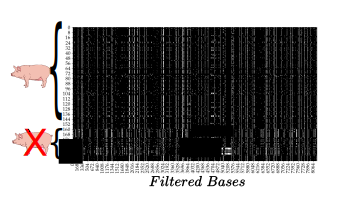
\includegraphics[width=0.85\textwidth]{Sequences.png}
\caption{SNP sequences of Salmonella enterica samples used in this work.
The x-axis shows the genome bases and the y-axis the corresponding sample (210 samples in total).
The black dots are related to a base without mutation (in relation to the genome reference), while the with dots are the mutation (SNPs) identified.
The first 159 rows contains the genome sequences related to pigs, i.e the sequences obtained by a pig which host the bacteria, and the following ones contains sequences of other animals.
Also with naked eyes we can see the differences between the two data types.
}
\label{fig:SNPsAle}
\end{figure}

First of all, we filtered our data removing from each genome a base if it was not mutated in each sample.
In this way we reduced the number of bases to $8189\,bp$.
A graphical representation of these samples is given in Fig.~\ref{fig:SNPsAle}.
The dataset was divided in training and test sets using a stratified cross-validation procedure to guarantee a proportional subdivision of the samples into the two classes.
The algorithm hyper-parameters were tuned on the training set in relation to the performances obtained using a internal stratified 10-fold cross-validation: in each fold the training was performed using a sequence of hyper-parameters and the performances evaluated on the corresponding test set; the hyper-parameters configuration which obtained the best performances on the full training set was chosen as best one.
We use our custom \emph{Score} library for the performance evaluation.
Considering the unbalanced sample quantities the Matthews Correlation Coefficient (MCC) was chosen as good score indicator for the evaluation.

\end{document}

\documentclass{standalone}

\begin{document}


\section[Conclusion]{Conclusion}\label{snp_conclusion}



\end{document}


\documentclass{standalone}

\begin{document}

\section[Byron]{Build YouR Own Neural network - Byron library}\label{byron}

Limits of the most common neural network frameworks.
Neural Network library for parallel computing developed in C++.
Pyron as python wrap of the library.
Description of the algorithms used to optimize the computation (ex. im2col vs winograd).


\end{document}


\documentclass{standalone}

\begin{document}

\section[Yolo]{Object Detection - Yolo architecture}\label{yolo}

%Introduction on the image classification and detection with Yolo architecture.
%Implementation in Byron with description of performances against darknet (original implementation).
%Focus on performances (time, memory, cpu).


\end{document}


\documentclass{standalone}

\begin{document}

\section[Super Resolution]{Super Resolution}\label{SR:sr}

\begin{figure}[htbp]
\def\svgwidth{0.5\textwidth}
\input{./img/sr_wow.pdf_tex}
\quad
\def\svgwidth{0.5\textwidth}
\input{./img/sr_wow2.pdf_tex}
\caption{Single Image Super Resolution.
Between the red lines the super resolved version of the image.
}
\label{fig:sr_wow}
\end{figure}

The Super Resolution (SR) is a slight novel technique based on Neural Network models which aims to improve the spatial resolution of a given image\footnote{
  The best-known \quotes{implementation} of Super Resolution concerns the microscopy super-resolution.
  In this work we are focusing on algorithms and numerical implementation so we will talk about the numerical counterpart of this technique, totally ignoring the original \quotes{hardware} version.
}.

The first SR methods on digital images estimate the high frequency information of the images starting from a series of low-resolution (LR) patches and their high-resolution (HR) counterpart.
These patches (ROIs of the LR image commonly smaller than $50\times50$) were extracted after an edge enhancement procedure or a simple 2D Fourier transform which extract the high frequency information.
Collecting these patches an \quotes{association dictionary} between LR and HR was created.
This dictionary was so used to learn the correct association between the LR e HR counterpart and then applied on new images.
The considered images could also be of the same dimensions in these firstly applications, i.e the purpose was only to improve the spatial resolution of the image without changing the sampling step.

The idea of use neural network models and in particular convolution functions to face on this problem was born in 2014 at the Engineering University of Honk Kong due to the large popularity of these models during that years.
The increasing computational power allowed to create automatic models able to learn the LR-HR association without any dictionary.
In this year arise the SRCNN model~\cite{SRCNN}, a three-layer neural network able to learn a large ensemble of features to reproduce the desired association.
The first layer aimed to extract the LR patches from the input image; the second layer produce the association between the LR patches and the tuned HR ones; the last layer reorganized the HR patches ensemble produced into a single HR image, i.e the output.

From this starting implementation many improvements was performed in this research field but the fundamental idea is not changed.
Modern models simply have a greater number of layers, due to the increasing computational power availability, and they used appropriate workaround to overcome the (large-)parameters tuning problem.

In the next sections we will show the super resolution technique step-by-step starting from the image pre-processing until the most modern algorithmic solutions.
At the end of this chapter the \textsf{NumPyNet} and \textsf{Byron} implementation of some modern models will be presented and applied over biomedical images.

%Introduction on Super Resolution problem with focus on state-of-art neural network architecture.
%Description of the Byron implementation and application on NMR data with the most common measurements.
%Super-resolution allows better detection!


\end{document}


\documentclass{standalone}

\begin{document}

\section[Segmentation]{Image Segmentation}\label{segmentation:unet}

\begin{center}
\begin{figure}[htbp]
\centering
\includegraphics[width=0.85\textwidth]{segmentation.jpg}
\label{fig:segmentation}
\end{figure}
\end{center}

In the previous section we have discussed about the object classification and object detection problems (ref.~\ref{obj_detection:obj}).
Now we want to go deeper on this topic and extract the exact pixels which belong to an object into a given image.
This kind of problem is called Image Segmentation, i.e give a label to each pixel of the input image.

Image segmentation is a typical task in many research fields and could be used for different purposes.
information about pixel-wise position of objects inside an image could be used for extract object shapes from the image or to simplify and/or change the representation of an image into something more meaningful and easier to understand.
This is an hot topic especially for self-driving car applications in which we have to find the exact shapes of object to better estimate their perspective position.
Moreover, all these applications require fast algorithm as much as possible closed to real-time.

This kind of task can be performed using a pipeline of image processing functions or by training a neural network model.
In the first case we have to stack a series of function to process the input image: it has to filters and extracts the useful information about the searched object but most of all it has to be as most general as possible to face on the common heterogeneity of samples.
In the second case we leave to the neural network model parameters the searching of optimal combination of function but we have to provide a supervised input pattern, i.e a combination of input and annotated pixel-wise mask of each image.
The image annotation is one of the most hardest and boring step of image segmentation and for these reasons is very hard to find public dataset usable.

In this chapter we introduce a particular neural network model commonly used in image segmentation problems and we will describe its characteristics and performances.
We applied this model to a novel dataset of CT images.
The dataset annotation was performed by a custom semi-supervised pipeline of image processing and the neural network model was trained and tested on this dataset.
The original data are taken from \href{https://mrl.sci.utah.edu/software/normal-hip-image-data/}{here}~\cite{doi:10.1002/jor.22040} and the corresponding annotations are released on \href{}{here}. % TODO: add google-drive link

\end{document}



\end{document}

% Description of the modern deep neural networks with potential applications
% Neural Network laboratory developed in pure numpy. Study of the neural network functionality and testing of the code against tensorflow
% rFBP library to optimize the Julia code with reference to the Scorer library and application to COMPARE data (Daniele Thesis)
% Neural Network library for parallel computing developed in C++ with python wrap. Description of the algorithms and strategies chosen in the library development.
% Introduction on the image classification and detection with Yolo architecture. Implementation in Byron with description of performances against darknet (original implementation). Focus on performances (time, memory, cpu).
% Introduction on Super Resolution problem with focus on state-of-art neural network architecture. Description of the Byron implementation and application on NMR data with the most common measurements. Super-resolution allows better detection!
% Introduction on Image Segmentation problem and application of Unet (Byron implementation) on femur images (TODO)


%% Chapter 3 - CHIMeRA project

\documentclass{standalone}

\begin{document}


\documentclass{standalone}

\begin{document}

\chapter[Big Data]{Biological Big Data - CHIMeRA project}\label{chapter3:bigdata}

The increasing availability of large-scale biomedical literature under the form of public on-line databases, has opened the door to a whole new understanding of multi-level associations between genomics, protein interactions and metabolic pathways for human diseases via network approaches.
Many structures and resources aiming at such type of analyses have been built, with the purpose of disentangling the complex relationships between various aspects of the human system relating to diseases~\cite{SymtomsNet, HumanPhenotype}.


%talk about data structured and unstructured
%Many public datasets available.
%Description of the database used in chimera.
%Problems about the intersections and partial informations (single db).


\end{document}


\documentclass{standalone}

\begin{document}

\section[CHIMeRA]{The CHIMeRA project}\label{chimera:chimera}

The increasing availability of large-scale biomedical literature under the form of public on-line databases, has opened the door to a whole new understanding of multi-level associations between genomics, protein interactions and metabolic pathways for human diseases via network approaches.
Many structures and resources aiming at such type of analyses have been built, with the purpose of disentangling the complex relationships between various aspects of the human system relating to diseases~\cite{SymtomsNet, HumanPhenotype}.
All these data come from different kind of studies performed by independent research groups who want to prove their theory about a particular aspect of the human biological interactions.
The capillarity of biological analyses allow to focus on a very deep aspect of these relationships, completely ignoring all the other agents.
This approach is certainly extremely efficient for the detection of the minimal causal agents of the problem but it tends to loose the global and complex\footnote{
  From a physical point-of-view.
} environment and prospective in which the process occurs.
The study of individual aspects concerning a particular disease could give us only a partial overview of the problem and the merge of the various research study it is hard to perform.

The network structures are acquiring even more importance on this kind of studies.
Complex System and System Biology researches have proposed multiple models about the dynamical and evolutionary interactions of the human system agents aiming to study the hidden relations between them.
A network model, in fact, is able to highlight and quantify the non-trivial correlations between our data.
The main problem of this kind of approach is certainly the increasing dimensionality of the involved data: a network model could be described via its adjacency matrix, i.e a matrix $(N\times N)$ in which each row/column identifies an agent of the understudy problem and each entry $(i, j)$ quantifies the importance of the interaction between the agent $i$ and the agent $j$.
In real data applications we can often reasonably assume that a wide amount of the matrix entries are null, i.e the interaction between the involved agent is quite sparse, and thus we can used the important properties related to the sparse matrices.
However, when the amount of data increase also the management of a such sparse matrix could be difficult.
More efficient solutions are provided by the modern Database formats and languages (e.g MySQL, SQLite, InfluxDB, $\cdots$) which store all these informations into a binary format and they allow to submit queries to extract the desired portion of data.
A global visualization of these huge amount of data is, in fact, without practical-sense and none valuable informations can extract from the global representation of the model.

In light of these considerations we started to develop the CHIMeRA project (\emph{Complex Human Interactions in MEdical Records and Atlases}) in which we aim to merge the state-of-art studies and databases about biomedical agents into a unified network structure.
A key role on our network structure is played by the diseases: the major part of biological researches are focused on causes and consequences of a given disease and thus the corresponding databases involve the interaction between them and other biological factors.
The diseases are also the most bigger manifestations of biological malfunctions and the large part of biological researches are financed on their study.
Thus a disease could be a valid \quotes{bridge} between multiple data sources which highlights the multiple biological aspects related to it.

The crucial point of this project was, in fact, the merging of different kind of informations provided by multiple distinct data structured.
As told above, the major part of researches focus on a partial aspect of the problem and they provide an independent result from the others, reducing the possibility of interactions between the outputs.
Moreover, a lot of time is always spent for the creation of a practical visualization of the results using web pages and on-line services which drastically affect the real usage of these informations when we want to combine multiple sources.
The CHIMeRA project started from these independent sources and it aims to maximize the overlap and thus the communications between them.
Multiple language databases were used to fill the gaps between the different biological ones.
%TODO : finire


%What is CHIMeRA project and which is its potentiality.
%Description of the database created and of the query implemented to obtain the results %TODO: better query


\end{document}

\documentclass{standalone}

\begin{document}

\section[CHIMeRA]{The CHIMeRA project}\label{chimera:chimera}

The increasing availability of large-scale biomedical literature under the form of public on-line databases, has opened the door to a whole new understanding of multi-level associations between genomics, protein interactions and metabolic pathways for human diseases via network approaches.
Many structures and resources aiming at such type of analyses have been built, with the purpose of disentangling the complex relationships between various aspects of the human system relating to diseases~\cite{SymtomsNet, HumanPhenotype}.
All these data come from different kind of studies performed by independent research groups who want to prove their theory about a particular aspect of the human biological interactions.
The capillarity of biological analyses allow to focus on a very deep aspect of these relationships, completely ignoring all the other agents.
This approach is certainly extremely efficient for the detection of the minimal causal agents of the problem but it tends to loose the global and complex\footnote{
  From a physical point-of-view.
} environment and prospective in which the process occurs.
The study of individual aspects concerning a particular disease could give us only a partial overview of the problem and the merge of the various research study it is hard to perform.

The network structures are acquiring even more importance on this kind of studies.
Complex System and System Biology researches have proposed multiple models about the dynamical and evolutionary interactions of the human system agents aiming to study the hidden relations between them.
A network model, in fact, is able to highlight and quantify the non-trivial correlations between our data.
The main problem of this kind of approach is certainly the increasing dimensionality of the involved data: a network model could be described via its adjacency matrix, i.e a matrix $(N\times N)$ in which each row/column identifies an agent of the understudy problem and each entry $(i, j)$ quantifies the importance of the interaction between the agent $i$ and the agent $j$.
In real data applications we can often reasonably assume that a wide amount of the matrix entries are null, i.e the interaction between the involved agent is quite sparse, and thus we can used the important properties related to the sparse matrices.
However, when the amount of data increase also the management of a such sparse matrix could be difficult.
More efficient solutions are provided by the modern Database formats and languages (e.g MySQL, SQLite, InfluxDB, $\cdots$) which store all these informations into a binary format and they allow to submit queries to extract the desired portion of data.
A global visualization of these huge amount of data is, in fact, without practical-sense and none valuable informations can extract from the global representation of the model.

In light of these considerations we started to develop the CHIMeRA project (\emph{Complex Human Interactions in MEdical Records and Atlases}) in which we aim to merge the state-of-art studies and databases about biomedical agents into a unified network structure.
A key role on our network structure is played by the diseases: the major part of biological researches are focused on causes and consequences of a given disease and thus the corresponding databases involve the interaction between them and other biological factors.
The diseases are also the most bigger manifestations of biological malfunctions and the large part of biological researches are financed on their study.
Thus a disease could be a valid \quotes{bridge} between multiple data sources which highlights the multiple biological aspects related to it.

The crucial point of this project was, in fact, the merging of different kind of informations provided by multiple distinct data structured.
As told above, the major part of researches focus on a partial aspect of the problem and they provide an independent result from the others, reducing the possibility of interactions between the outputs.
Moreover, a lot of time is always spent for the creation of a practical visualization of the results using web pages and on-line services which drastically affect the real usage of these informations when we want to combine multiple sources.
The CHIMeRA project started from these independent sources and it aims to maximize the overlap and thus the communications between them.
Multiple language databases were used to fill the gaps between the different biological ones.
%TODO : finire


%What is CHIMeRA project and which is its potentiality.
%Description of the database created and of the query implemented to obtain the results %TODO: better query


\end{document}

\documentclass{standalone}

\begin{document}

\section[CHIMeRA]{The CHIMeRA project}\label{chimera:chimera}

The increasing availability of large-scale biomedical literature under the form of public on-line databases, has opened the door to a whole new understanding of multi-level associations between genomics, protein interactions and metabolic pathways for human diseases via network approaches.
Many structures and resources aiming at such type of analyses have been built, with the purpose of disentangling the complex relationships between various aspects of the human system relating to diseases~\cite{SymtomsNet, HumanPhenotype}.
All these data come from different kind of studies performed by independent research groups who want to prove their theory about a particular aspect of the human biological interactions.
The capillarity of biological analyses allow to focus on a very deep aspect of these relationships, completely ignoring all the other agents.
This approach is certainly extremely efficient for the detection of the minimal causal agents of the problem but it tends to loose the global and complex\footnote{
  From a physical point-of-view.
} environment and prospective in which the process occurs.
The study of individual aspects concerning a particular disease could give us only a partial overview of the problem and the merge of the various research study it is hard to perform.

The network structures are acquiring even more importance on this kind of studies.
Complex System and System Biology researches have proposed multiple models about the dynamical and evolutionary interactions of the human system agents aiming to study the hidden relations between them.
A network model, in fact, is able to highlight and quantify the non-trivial correlations between our data.
The main problem of this kind of approach is certainly the increasing dimensionality of the involved data: a network model could be described via its adjacency matrix, i.e a matrix $(N\times N)$ in which each row/column identifies an agent of the understudy problem and each entry $(i, j)$ quantifies the importance of the interaction between the agent $i$ and the agent $j$.
In real data applications we can often reasonably assume that a wide amount of the matrix entries are null, i.e the interaction between the involved agent is quite sparse, and thus we can used the important properties related to the sparse matrices.
However, when the amount of data increase also the management of a such sparse matrix could be difficult.
More efficient solutions are provided by the modern Database formats and languages (e.g MySQL, SQLite, InfluxDB, $\cdots$) which store all these informations into a binary format and they allow to submit queries to extract the desired portion of data.
A global visualization of these huge amount of data is, in fact, without practical-sense and none valuable informations can extract from the global representation of the model.

In light of these considerations we started to develop the CHIMeRA project (\emph{Complex Human Interactions in MEdical Records and Atlases}) in which we aim to merge the state-of-art studies and databases about biomedical agents into a unified network structure.
A key role on our network structure is played by the diseases: the major part of biological researches are focused on causes and consequences of a given disease and thus the corresponding databases involve the interaction between them and other biological factors.
The diseases are also the most bigger manifestations of biological malfunctions and the large part of biological researches are financed on their study.
Thus a disease could be a valid \quotes{bridge} between multiple data sources which highlights the multiple biological aspects related to it.

The crucial point of this project was, in fact, the merging of different kind of informations provided by multiple distinct data structured.
As told above, the major part of researches focus on a partial aspect of the problem and they provide an independent result from the others, reducing the possibility of interactions between the outputs.
Moreover, a lot of time is always spent for the creation of a practical visualization of the results using web pages and on-line services which drastically affect the real usage of these informations when we want to combine multiple sources.
The CHIMeRA project started from these independent sources and it aims to maximize the overlap and thus the communications between them.
Multiple language databases were used to fill the gaps between the different biological ones.
%TODO : finire


%What is CHIMeRA project and which is its potentiality.
%Description of the database created and of the query implemented to obtain the results %TODO: better query


\end{document}

\end{document}

% Many public datasets available. Description of the database used in chimera
% Description of the web scraping techinques used to obtain the "no-public" datasets. Reference to the github project
% What is CHIMeRA project and which potentiality it has. Description of the database created and of the query implemented to obtain the results (TODO: better query)
% Some query examples like leukemia subnetwork and PRNP subnetwork. Description of the information extracted by these subnetworks


%% Chapter 4 - cardiological data

% \input{./tex/Chapter4/AppitechData.tex}
% % Description of the pulsoximmetry and of the cardiological data analyzed

% \input{./tex/Chapter4/CardioFeature.tex}
% % Description of the features extracted on the cardiological dataset

% \input{./tex/Chapter4/AgePrediction.tex}
% % Pipeline of the feature selection with age prediction obtained on cardio data

%% Conclusion

\documentclass{standalone}

\begin{document}

\chapter*{Conclusions}\label{conclusions}\addcontentsline{toc}{chapter}{Conclusions}



\end{document}


%% Acknowledgment

\pagenumbering{gobble}% Remove page numbers (and reset to 1)
\documentclass{standalone}

\begin{document}

\chapter*{Acknowledgment}

\end{document}


%% Appendix

\documentclass{standalone}

\begin{document}

\documentclass{standalone}

\begin{document}

\chapter*{Appendix A - Discriminant Analysis}\addcontentsline{toc}{chapter}{Appendix A - Discriminant Analysis}
\markboth{Appendix A}{Discriminant Analysis}

The classification problems aim to associate a set of \emph{pattern} to one or more \emph{classes}.
With \emph{pattern} we identify a multidimensional array of data labeled by a pre-determined tag.
In this case we talk about \emph{supervised learning}, i.e the full set of data is already annotated and we have prior knowledge about data association to the belonging classes.
Since in this work only supervised learning algorithms have been analyzed we do not cite other different learning methods.

In machine learning a key rule is assumed by Bayesian methods, i.e methods which use a Bayesian statistical approach to the analysis of data distributions.
It can be proof that if the distributions under analysis are known, i.e a sufficient number of moments of it is known with a sufficient precision, the Bayesian approach is the best possible method to face on the classification problem. % cite!

\end{document}

\input{./tex/Appendix/DiscriminantAnalysis/MathematicalBackground.tex}
\documentclass{standalone}

\begin{document}

\section*{Numerical Implementation}\addcontentsline{toc}{section}{Numerical Implementation}
\markboth{Appendix A}{Numerical Implementation}

From a computational point-of-view we can exploit each mathematical information and assumption to simplify the computation and improve the numerical stability of our computation.
We would remark that these considerations were taken into account in this work only for the \textsf{C++} algorithmic implementation, since these methods are already implemented in high-level programming languages as \textsf{Python} and \textsf{Matlab}\footnote{
  For sake of completeness we have to highlight that the classification functions provided by \textsf{Matlab}, i.e \textsf{classify}, are already included into the base software packages, i.e no external Toolbox is needed, while for the \textsf{Python} case the most common package which implements these techniques is given by the \textsf{scikit-learn} library.
  \textsf{Matlab} allows to set the classifier type as input parameter of the function using a simple string which follows the same nomenclature previously proposed.
  \textsf{Python} has a different imports for each classifier type: in this case we found correspondence between our nomenclature and the \textsf{Python} one only in \emph{quadratic} and \emph{linear} cases, while the \emph{Mahalanobis} classifier is not considered as putative classifier.
  The \emph{diagquadratic} classifier is called \textsf{GaussianNB} (\emph{Naive Bayes Classifier}) instead.
  The last important discrepancy between the two language implementations is found in variance evaluation (and corresponding covariance matrix): \textsf{Matlab} proposes the variance estimation only in relation to the mean so the normalization coefficient is given by the number of samples except by one ($N-1$), while \textsf{Python} computes the variance with a simple normalization by $N$.
}.

In the previous section we highlighted the covariance matrix properties, i.e the covariance matrix is a positive semi-definite and symmetric matrix by definition and these properties allow the matrix inversion.
The computation of the inverse-matrix is a well known complex computational step from a numerical point-of-view and in a general case can be classified as an $O(N^3)$ algorithm.
Moreover, the usage of a Machine Learning classifier commonly matches the usage of a cross validation method, i.e multiple subdivision of the dataset into training and test sets.
This involves the computation of multiple inverse matrices and it could represents the performance bottleneck in many real applications (the other computations are quite simple and their algorithmic complexity are certainly less than $O(N^3)$).

Using the mathematical information about covariance matrix we can find the best numerical solution for its inverse that in this case is given by the Cholesky decomposition algorithm.
The Cholesky decomposition or Cholesky factorization allows to rewrite a positive-definite matrix into the product of two triangular matrices (the first is the conjugate transposed of the second)

$$
\mathbf{A} = \mathbf{LL^T} = \mathbf{U^TU}
$$
\\
The algorithmic complexity is still the same but the inverse estimation is simpler using a triangular matrix and the entire inversion can be performed in-place.
It can also be proved that general inverse matrix algorithms suffer of numerical instability issues compared to the output of Cholesky decomposition.
In this case the original inverse matrix can be computed by the multiplication of the two inverses as

$$
\mathbf{A^{-1}} = (\mathbf{L^{-1}})^T(\mathbf{L^{-1}}) = (\mathbf{U^{-1}})(\mathbf{U^{-1}})^T
$$
\\
As second bonus, cross validation methods involve the data splitting in multiple non-independent chunks of the original data.
The extreme case of this algorithm is given by the Leave-One-Out cross validation in which the data superposition between folds is $N-1$ (where $N$ is the size of the data).
The statistical influence of the swapped data is quite low and the covariance matrix would be quite similar across folds (the inverse matrix would be drastically affected from each slight modification of the original matrix instead).
A second step of optimization can be performed computing the original full-covariance matrix of the whole set of data ($O(N^2)$) and modify it into the right $k$ indexes at each cross-validation step ($O(N*k)$) that in the Leave-One-Out become a single editing case.
This second optimization  can also be performed in the Diag-Quadratic case substituting the covariance matrix with the simpler variance vector.

% maybe insert some code snippets

Both these two techniques have been used in the \textsf{C++} implementation of the Quadratic Discriminant Analysis classifier and in the Diag-Quadratic Discriminant Analysis classifier used in the \textsf{DNetPRO} algorithm implementation (see~\ref{dnetpro:DNetPRO}).


\end{document}



\documentclass{standalone}

\begin{document}

\section[CHIMeRA]{The CHIMeRA project}\label{chimera:chimera}

The increasing availability of large-scale biomedical literature under the form of public on-line databases, has opened the door to a whole new understanding of multi-level associations between genomics, protein interactions and metabolic pathways for human diseases via network approaches.
Many structures and resources aiming at such type of analyses have been built, with the purpose of disentangling the complex relationships between various aspects of the human system relating to diseases~\cite{SymtomsNet, HumanPhenotype}.
All these data come from different kind of studies performed by independent research groups who want to prove their theory about a particular aspect of the human biological interactions.
The capillarity of biological analyses allow to focus on a very deep aspect of these relationships, completely ignoring all the other agents.
This approach is certainly extremely efficient for the detection of the minimal causal agents of the problem but it tends to loose the global and complex\footnote{
  From a physical point-of-view.
} environment and prospective in which the process occurs.
The study of individual aspects concerning a particular disease could give us only a partial overview of the problem and the merge of the various research study it is hard to perform.

The network structures are acquiring even more importance on this kind of studies.
Complex System and System Biology researches have proposed multiple models about the dynamical and evolutionary interactions of the human system agents aiming to study the hidden relations between them.
A network model, in fact, is able to highlight and quantify the non-trivial correlations between our data.
The main problem of this kind of approach is certainly the increasing dimensionality of the involved data: a network model could be described via its adjacency matrix, i.e a matrix $(N\times N)$ in which each row/column identifies an agent of the understudy problem and each entry $(i, j)$ quantifies the importance of the interaction between the agent $i$ and the agent $j$.
In real data applications we can often reasonably assume that a wide amount of the matrix entries are null, i.e the interaction between the involved agent is quite sparse, and thus we can used the important properties related to the sparse matrices.
However, when the amount of data increase also the management of a such sparse matrix could be difficult.
More efficient solutions are provided by the modern Database formats and languages (e.g MySQL, SQLite, InfluxDB, $\cdots$) which store all these informations into a binary format and they allow to submit queries to extract the desired portion of data.
A global visualization of these huge amount of data is, in fact, without practical-sense and none valuable informations can extract from the global representation of the model.

In light of these considerations we started to develop the CHIMeRA project (\emph{Complex Human Interactions in MEdical Records and Atlases}) in which we aim to merge the state-of-art studies and databases about biomedical agents into a unified network structure.
A key role on our network structure is played by the diseases: the major part of biological researches are focused on causes and consequences of a given disease and thus the corresponding databases involve the interaction between them and other biological factors.
The diseases are also the most bigger manifestations of biological malfunctions and the large part of biological researches are financed on their study.
Thus a disease could be a valid \quotes{bridge} between multiple data sources which highlights the multiple biological aspects related to it.

The crucial point of this project was, in fact, the merging of different kind of informations provided by multiple distinct data structured.
As told above, the major part of researches focus on a partial aspect of the problem and they provide an independent result from the others, reducing the possibility of interactions between the outputs.
Moreover, a lot of time is always spent for the creation of a practical visualization of the results using web pages and on-line services which drastically affect the real usage of these informations when we want to combine multiple sources.
The CHIMeRA project started from these independent sources and it aims to maximize the overlap and thus the communications between them.
Multiple language databases were used to fill the gaps between the different biological ones.
%TODO : finire


%What is CHIMeRA project and which is its potentiality.
%Description of the database created and of the query implemented to obtain the results %TODO: better query


\end{document}
\documentclass{standalone}

\begin{document}

\section*{The datasets}\addcontentsline{toc}{section}{The datasets}
\markboth{Appendix B}{The datasets}

The dataset used in this study has been provided by the Italian mobile phone company TIM and contains geo-referenced positions of tens of thousands anonymous devices (e.g. mobile phones, tablets, etc. ...), whenever they performed an activity (e.g. a phone call or an Internet access) during eight days from 23/2/2017 up to 02/03/2017 (Carnival of Venice dataset), and from 14/7/2017 up to 16/7/2017 (\emph{Festa del Redentore} dataset).
According to statistical data, 66\% of the whole Italian population has a smart-phone and TIM is one the greatest mobile phone company in Italy whose users are $\sim30\%$ of the whole smart-phone population.
The datasets refer to a geographical region that includes an area of the Venice province, so that it is possible to distinguish commuters from sedentary people and the different transportation means used to reach Venice.
Each valid record gives information about the GPS localization of the device, the recording time, the signal quality and also the roaming status, which in turns allow to distinguish between Italian and
foreigners.
The devices are fully anonymized and not reversible identification numbers (ID) are automatically provided by the system for mobile phones and calls within the scope of the trial; the ID is kept for a period of 24 hours.
During each activity a sequence of GPS data is recorded with a 2 sec. sampling rate and the collection stops when the activity ends.
As matter of fact during an activity most of people reduce their mobility except if they are on a transportation mean, so that the dataset contains a lot of small trajectories that have to be joined to reconstruct the daily mobility.
After a filtering procedure these data provide information on the mobility of a sample containing 3000~–~4000 devices per day.
Since the presences during the considered events were of the order of 105 individuals per day, as reported by the local newspapers, we estimate an overall penetration of our sample of 3~–~4\%.
The filtering procedure and the other statistical informations about the sample penetration are discussed in the original paper~\cite{Mizzi2018}.

\end{document}
\input{./tex/Appendix/Venice/MobilityPaths.tex}


\documentclass{standalone}

\begin{document}

\chapter*{Appendix C - BlendNet}\addcontentsline{toc}{chapter}{Appendix C - BlendNet}
\markboth{Appendix C}{BlendNet}

\begin{figure}[htbp]
\centering
\includegraphics[width=0.4\textwidth]{cycle_graph.png}
\qquad\qquad
\includegraphics[width=0.4\textwidth]{star_graph_node.png}
\caption{(\textbf{a}) Chain graph rendered by \textsf{BlendNet} software.
Node colors are randomly generated by the tool.
(\textbf{b}) Star graph rendered by \textsf{BlendNet} software.
Node colors and labels are given as extra columns in node-list file.
}
\label{fig:blendnet}
\end{figure}

Graph visualization is still an open problem in many applications.
The problem is commonly related to large graph visualization in which problems arise from the rendering of a large number of nodes and a greater number of links between them (a graph with $N$ nodes could have $(N \times N)$ possible links).
An other open problem concern the multi-dimensional visualization of the graphs.
Despite common graph tools compute the node coordinates in any space dimensions (and clearly the maximum number of possible dimensions for a visualization is only 3) the real visualization is often allowed only in 2D spaces.
The counterpart of these problems concern a pretty visualization of the graphs, that it is often ignored by many tools which prefer focusing on simple renderings.

In this section we introduce a new custom graph viewer developed for pretty small-networks visualization in 2D and 3D, called \href{https://github.com/Nico-Curti/BlendNet}{\textsf{BlendNet}}~\cite{BlendNet} (\emph{Blender Network viewer}).
\textsf{BlendNet} is an open-source project and it is released on Github under GPL license.
All the small-graphs showed in this work are made using this tool and in particular the feature-signatures generated by the \textsf{DNetPRO} algorithm.

\textsf{BlendNet} is written in \textsf{Python} with the help of \textsf{Blender} APIs.
\textsf{Blender} is now a standard for 3D rendering and it is commonly used in a wide range of graphical applications, starting from the simpler 3D dynamics to video-game applications.
\textsf{Blender} is certainly more than a simple graphical viewer, but it provides an easy \textsf{Python} interface and a wide on-line documentation which make it a useful tool for graphical representation of 3D structures.

We are forced to use the \textsf{Python} version provided by \textsf{Blender} to use its APIs and any extra-package required by our application has to be installed with the appropriated \textsf{pip}.
We use the \textsf{networkx} \textsf{Python} library for node coordinates computation and thus we have to update our \textsf{Python}-\textsf{Blender} with the appropriated packages.
Moreover, since the code can be difficult to manage for non-expert users, we have written an easy command-line interface to set the whole set of parameters required by the graph viewer that can be piloted via \href{https://github.com/Nico-Curti/BlendNet/blob/master/Makefile}{\textsf{Makefile}} rules.
The list of nodes and edges can be passed via command-line with the relative filenames, in the same format of the concurrent graph viewers (e.g \emph{Gephi} software, the other graph viewer used in this work to generate the larger network structures of the \textsf{CHIMeRA} project).

The software project is a single script file and it includes a full list of possible \href{https://github.com/Nico-Curti/BlendNet/blob/master/example}{examples} and usages.
Some of this examples are shown in Fig.~\ref{fig:blendnet}.
A full list of installation instructions is also provided for any operative system (\href{https://github.com/Nico-Curti/BlendNet/blob/master/install.sh}{Unix, MacOS} and \href{https://github.com/Nico-Curti/BlendNet/blob/master/install.ps1}{Windows}).
These instructions cover a full installation of \textsf{Blender}, \textsf{Python} and \textsf{BlendNet} package for administrator and no-root users (ref. \textsf{Shut} project \cite{Shut}).
With slight code editing we can obtain different node coordinates and shapes.
Node colors, sizes and positions can also be given using the node-list file as independent columns.

\end{document}


\documentclass{standalone}

\begin{document}

\section[CHIMeRA]{The CHIMeRA project}\label{chimera:chimera}

The increasing availability of large-scale biomedical literature under the form of public on-line databases, has opened the door to a whole new understanding of multi-level associations between genomics, protein interactions and metabolic pathways for human diseases via network approaches.
Many structures and resources aiming at such type of analyses have been built, with the purpose of disentangling the complex relationships between various aspects of the human system relating to diseases~\cite{SymtomsNet, HumanPhenotype}.
All these data come from different kind of studies performed by independent research groups who want to prove their theory about a particular aspect of the human biological interactions.
The capillarity of biological analyses allow to focus on a very deep aspect of these relationships, completely ignoring all the other agents.
This approach is certainly extremely efficient for the detection of the minimal causal agents of the problem but it tends to loose the global and complex\footnote{
  From a physical point-of-view.
} environment and prospective in which the process occurs.
The study of individual aspects concerning a particular disease could give us only a partial overview of the problem and the merge of the various research study it is hard to perform.

The network structures are acquiring even more importance on this kind of studies.
Complex System and System Biology researches have proposed multiple models about the dynamical and evolutionary interactions of the human system agents aiming to study the hidden relations between them.
A network model, in fact, is able to highlight and quantify the non-trivial correlations between our data.
The main problem of this kind of approach is certainly the increasing dimensionality of the involved data: a network model could be described via its adjacency matrix, i.e a matrix $(N\times N)$ in which each row/column identifies an agent of the understudy problem and each entry $(i, j)$ quantifies the importance of the interaction between the agent $i$ and the agent $j$.
In real data applications we can often reasonably assume that a wide amount of the matrix entries are null, i.e the interaction between the involved agent is quite sparse, and thus we can used the important properties related to the sparse matrices.
However, when the amount of data increase also the management of a such sparse matrix could be difficult.
More efficient solutions are provided by the modern Database formats and languages (e.g MySQL, SQLite, InfluxDB, $\cdots$) which store all these informations into a binary format and they allow to submit queries to extract the desired portion of data.
A global visualization of these huge amount of data is, in fact, without practical-sense and none valuable informations can extract from the global representation of the model.

In light of these considerations we started to develop the CHIMeRA project (\emph{Complex Human Interactions in MEdical Records and Atlases}) in which we aim to merge the state-of-art studies and databases about biomedical agents into a unified network structure.
A key role on our network structure is played by the diseases: the major part of biological researches are focused on causes and consequences of a given disease and thus the corresponding databases involve the interaction between them and other biological factors.
The diseases are also the most bigger manifestations of biological malfunctions and the large part of biological researches are financed on their study.
Thus a disease could be a valid \quotes{bridge} between multiple data sources which highlights the multiple biological aspects related to it.

The crucial point of this project was, in fact, the merging of different kind of informations provided by multiple distinct data structured.
As told above, the major part of researches focus on a partial aspect of the problem and they provide an independent result from the others, reducing the possibility of interactions between the outputs.
Moreover, a lot of time is always spent for the creation of a practical visualization of the results using web pages and on-line services which drastically affect the real usage of these informations when we want to combine multiple sources.
The CHIMeRA project started from these independent sources and it aims to maximize the overlap and thus the communications between them.
Multiple language databases were used to fill the gaps between the different biological ones.
%TODO : finire


%What is CHIMeRA project and which is its potentiality.
%Description of the database created and of the query implemented to obtain the results %TODO: better query


\end{document}

\documentclass{standalone}

\begin{document}

\chapter*{Appendix E - Neural Network as Service}\addcontentsline{toc}{chapter}{Appendix E - Neural Network as Service}
\markboth{Appendix E}{Neural Network as Service}

One of the final goals of Machine Learning is certainly the automation of the processes.
We develop complex models to perform tasks that can be automatically executed by a computer without human supervision.
Neural Networks are classically mathematical tools used for these purposes and was wide discussed in Chapter~\ref{chapter2:neural} of this work.
Beyond the Neural Network structures and purposes for which they are made there is a still uncovered topic to discuss: the automation of these kind of algorithms inside a computer device.
In this section we discuss an example of implementation of these algorithms as service in computer server.
In particular we will talk about the implementation of the \emph{FiloBlu} service which is a project developed in collaboration with the University of Sapienza (Roma) and the INFN-CNAF of Bologna.
Since this work is still in progress and its purpose goes beyond the current topic, we will focused only on the implementation of the service without any reference on the Machine Learning algorithm used.
This is a further proof that the developed techniques are totally independent by the final application purpose.

A service is a software that is executed in background in a machine.
In Unix machines it is often call \textsf{daemon} while in Windows machine is called \emph{Windows service}.
A service can be started only by admin users and it goes on without any user presence.
An other important requirement is the ability to re-start when some troubles occurs in the machine functionality and/or at the boot of the machine.

A Machine Learning service could be used in applications in which we have to manage an asynchronous stream of data for long time intervals.
An example could be the case which the data provider is identified by an App or a video-camera.
These data should stored inside a central database that can be located in a different device or in the same computer in which the service run.
Since the service process runs in background the only communication channel with the user is given by log files.
A log file is a simple readable file in which are saved the base informations about the current status of the service.
Thus, it is crucial to set appropriate check-points inside the service script and chose the minimum quantity of informations that the service should write to make user-understandable its status.

\end{document}

\documentclass{standalone}

\begin{document}


\section*{FiloBlu Service}\addcontentsline{toc}{section}{FiloBlu Service}
\markboth{Appendix E}{FiloBlus Service}

In the \emph{FiloBlu} project we have a stream of data provided by an external App that are stored in a central database server.
The Machine Learning service has to read the information in the database, to process them and finally write the results in the same database.
All these operations have to be performed with high frequency since the result of the algorithm are shown in a real-time application.
This frequency will be the clock-time of the process function, i.e at each time interval (as small as we like) the process task will be called and we have the desired results in output.
At the same time we have to be care of the time required by our Machine Learning algorithm: not all the algorithms can process data in real time and the process function frequency has to be less than the time required by the algorithm or we can lose some frequency clock.

The best efficiency by a service can be obtained splitting as much as possible the required functionality in small-and-easy tasks.
Small task can evaluated as independent functions with an associated frequency that in this case can be reduced as much as possible.
The \emph{FiloBlu} required functionality can be reviewed as a sequence of 3 fundamental steps and other 2 optional ones: read the data from the database, process the data with the Machine Learning algorithm and write the obtained results on the database are certainly the fundamental ones; update the Machine Learning model and clear old log files are optional steps.
To further improve the efficiency of the service we can give each independent step to a different thread.
The whole set of tasks will be piloted by a master thread given by the service itself.
In this way the service will be computational efficient and moreover it does not weight on the computer performances.
We have always take in mind that the computer which host the service have to be effected by the daemon process as less as possible either in memory either on computational point-of-view.
Now we only have to synchronize our steps with appropriate clock frequencies.

Let's start from the reading data function.
Since our data are assumed to be stored in a database this function have to perform a simple query and extract the latest data inserted.
Obviously the efficiency of the step is based on the efficiency of the chosen query.
The data extracted will be saved in a common container shared between the list of thread and thus belonging to the master.
The choice of an appropriate shared container is a second point to carefully take in mind.
This container should be light an thread-safe to avoid thread concurrency.
While the second request is implementation dependent the first one can be faced on using a FIFO container\footnote{
  FIFO container, i.e \emph{First-In-First-Out}, is a special data structure in which the first element added will be processed as first and then automatically removed from it.
}.
In this way we can ensure that the application will saved a fixed maximum of data and it will not occupy large portion of memory (RAM).

The second task is identified by the Machine Learning function which process the data.
The algorithm will take from the FIFO container of the previous step (if there is) and it will save the result in a second FIFO container for the next step.
The time frequency of the step is given by the time required by the Machine Learning algorithm.

The third step will keep the data from the FIFO container of results (if there is) and it performs a second query (a writing one in this case) to the database.
Also in this case the frequency is given by the efficiency of the chosen query.

The last two steps can be executed without press time requirements and are useful only on a large time scale.

Each step perform its independent logging on a single shared file.
If an error occurs the service logs the message and save the current log-file in a different location to prevent possible log-cleaning (optional step).
Then the service will be re-started.

% \begin{figure}[htbp]
% \centering
% \def\svgwidth{0.8\textwidth}
% \input{./img/FiloBlu.pdf_tex}
% \caption{
% }
% \label{fig:FiloBlu}
% \end{figure}

%The above computational scheme of the service is shown in Fig.~\ref{fig:FiloBlu}.

We implemented this type of service in pure Python~\cite{FiloBlu}.
The developed service was customize according to the server requirements of the project\footnote{
  The FiloBlu service is a Windows service and it can not run on Unix machines.
  Moreover the database used in the project is a MySQL one so the queries and the libraries used are compatible only with this kind of databases.
}.
We chose the Python language either for its simplicity in the code writing either for its thread native module which ensures a total thread-safety of each variable.
Using simple decorator we are able to run each function in a separate-detached thread as required by the previous instructions.
The project includes a documentation about its use (also in general applications) and it can be easily installed via \textsf{setup}.
In the \emph{FiloBlu} project we use a Neural Network algorithm written in \emph{Tensorflow}.
\emph{Tensorflow} does not allow to run background process directly so the problem was overcame using a direct call to a Python script which perform full list of steps into an infinite loop.
In this way the service can be re-started also if the process-service is killed.
The service can be driven using a simple \emph{Powershell} script provided in the project.

\end{document}

\documentclass{standalone}

\begin{document}

\section*{Data Transmission}\addcontentsline{toc}{section}{Data Transmission}
\markboth{Appendix E}{CryptoSocket}

In the above configuration we focused on the pipeline which processes the stream of data, ignoring any problem about the communication between the external device and the machine which hosts the service.
The \emph{FiloBlu} project uses an external APP to send data to the main server, so we have two systems which have to communicate between them automatically via Internet connection.
In general, we could manage sensitive data, that could be vulnerable using an Internet communication.
To face this problem we developed a simple TCP/IP client-server package which also supports a RSA cryptography, the \textsf{CryptoSocket} package~\cite{CryptoSocket}.

The communication security could be an important point in many research applications and a valid cryptography procedure is essential.
The RSA cryptography is considered one of the most secure cryptography algorithm for data transmission and it is quite easy to implement.
In the \textsf{CryptoSocket} package we implemented a simple wrap around the \textsf{socket} \textsf{Python} library to perform a serialization of our data which are (optionally) processed by our custom \href{https://en.wikipedia.org/wiki/RSA_(cryptosystem)}{RSA algorithm}.
In this way different kinds of data could be sent by the client at the same time.
The \href{https://github.com/Nico-Curti/CryptoSocket/blob/master/CryptoSocket/examples/client.py}{client} script could be adapted with slight modifications for any user need and also complex \textsf{Python} structures could be transmitted between two machines (to the \href{https://github.com/Nico-Curti/CryptoSocket/blob/master/CryptoSocket/examples/server.py}{server}).
The cryptography module was written in pure \textsf{C++} for computational efficiency and a \textsf{Cython} wrap was provided for pure-\textsf{Python} applications.
\textsf{CryptoSocket} has only demonstrative purpose and so it works only for a 1-by-1 data transmission (1 server and 1 client).

Since this second implementation could be used also for other applications it was treated as a separated project and it has its own open-source code.
The \textsf{CryptoSocket} package can be installed via \href{https://github.com/Nico-Curti/CryptoSocket/blob/master/CMakeLists.txt}{\textsf{CMake}} in any platform and operative system and a full list of installation instructions is provided in the project repository.
The continuous integration of the project is guaranteed by testing the package installation across multiple \textsf{C++} compilers and platforms via \href{https://github.com/Nico-Curti/CryptoSocket/blob/master/.travis.yml}{Travis CI} and \href{https://github.com/Nico-Curti/CryptoSocket/blob/master/appveyor.yml}{Appveyor CI}.

\end{document}



\documentclass{standalone}

\begin{document}

\chapter*{Appendix F - Bioinformatics Pipeline Profiling}\addcontentsline{toc}{chapter}{Appendix F - Bioinformatics Pipeline Profiling}
\markboth{Appendix F}{Profiling}

In this work many times we have talked about the performances evaluation of a scripts in terms of time performances and other system statistics.
The importance in the understanding the state of our infrastructure is essential not only for ensuring the reliability and stability of a software but also for a more efficiency use of the available resources.
In particular about what concern the memory, CPUs and diskIO management is useful to know the required amount of each step of our software to perform the better parallelization strategy.
Metrics represent the raw measurements of resource usage that are used by a software or a collection of them.
These might be low-level usage summaries provided by the operating system, or they can be higher-level types of data tied to the specific functionality or work of a component.
These kind of data could be collected and aggregated by a monitoring system like \href{https://github.com/influxdata/telegraf}{\emph{Telegraf}}\footnote{
  An automatic installation guide for Telegraf is provided in the Shut~\cite{Shut} project for any OS and also for no-root users.
}.
In general, the difference between metrics and monitoring mirrors the difference between data and information.
Monitoring takes metrics data, aggregates it, and presents it in various ways that allow humans to extract insights from the collection of individual pieces.

In this section we focused on the importance of software monitoring.
In particular we will talk about a work conducted in collaboration with INFN-CNAF of Bologna about the monitoring and the performance evaluation of a bioinformatics pipeline across various computational environments~\cite{EuroPar2018}.

In this work a previously published bioinformatics pipeline was reimplemented across various computational platforms, and the performances of its steps evaluated.
The tested environments were:
I) dedicated bioinformatics-specific server
II) low-power single node
III) HPC single node
IV) virtual machine.
The pipeline was tested on a use case of the analysis of a single patient to assess single-use performances, using the same configuration of the pipeline to be able to perform meaningful comparison and search the optimal environment/hybrid system configuration for biomedical analysis.
Performances were evaluated in terms of execution wall time, memory usage and energy consumption per patient.

\end{document}

\documentclass{standalone}

\begin{document}


\section*{GATK-LODn pipeline}\addcontentsline{toc}{section}{GATK-LODn pipeline}
\markboth{Appendix F}{GATK-LODn}

\begin{table*}
\centering
\begin{tabular}{lccccc}
\hline \rowcolor{darkgrayrow}
 & \textbf{Coverage} & \textbf{No. of} & \textbf{Read}   & \textbf{BAM file} & \textbf{NGS}\\
\rowcolor{darkgrayrow}
 &                   & \textbf{Reads}  & \textbf{Length} & \textbf{size}     & \textbf{size}\\
\hline
\textbf{Whole genome} & 37.7x & 975,000,000   & 115 & 82 GB  & 104 GB \\

\textbf{Whole genome} & 38.4x & 3,200,000,000 & 36  & 138 GB & 193 GB\\

\textbf{Exome}        & 40x   & 110,000,000   & 75  & 5.7 GB & 7.1 GB \\
\hline\\
\end{tabular}
\caption{Typical dataset size for a single patient of different types of next generation sequencing.
BAM file size refers to the size of the binary file containing the reads from the machine.}
\label{fig:wes_datasize}
\end{table*}

The pipeline used in this work, GATK-LODn, has been developed in 2016 by Do Valle et al.~\cite{DoValle2016}, and codifies a new approach aimed to Single Nucleotype Polimorphism (SNP) identification in tumors from Whole Exome Sequencing data (WES).
WES is a type of \quotes{next generation sequencing} data~\cite{Zwolak2008, Behjati2013, Shendure2008}, focused on the part of the genome that actually codifies proteins (the exome).
Albeit known that non-transcriptional parts of the genome can affect the dynamic of gene expression, the majority of cancers inducing mutations are known to be on the exome, thus WES data allow to focus the computational effort on the most interesting part of the genome.
Being the exome in human approximately 1\% of the total genome, this approach helps significantly in reducing the number of false positives detected by the pipeline.
The different sizes of next generation sequencing dataset are shown in Tab~\ref{fig:wes_datasize}.

The GATK-LODn pipeline is designed to combine results of two different SNP-calling softwares, GATK~\cite{McKenna2010} and MuTect~\cite{Cibulskis2013}.
These two softwares employ different statistical approaches for the SNP calling: GATK examines the healthy tissue and the cancerous tissue independently, and identifies the suspect SNPs by comparing them; Mutect compares healthy and cancerous tissues at the same time and has a more strict threshold of selection.
In identifying more SNPs, GATK has a higher true positive calling than Mutect, but also an higher number of false positives.
On the other end Mutect has few false positives, but often does not recognize known SNPs.
The two programs also call different set of SNPs, even when the set size is similar.
The pipeline therefore uses a combination of the two sets of chosen SNPs to select a single one, averaging the strictness of Mutect with the recognition of known variants of GATK.

The pipeline work-flow includes a series of common steps in bioinformatics analysis and in the common bioinformatics pipelines.
It includes also a sufficient representative sample of tools for the performances statistical analysis.
In this way the results extracted from the single steps analysis could be easily generalized to other standard bioinformatics pipelines.

With the increasing demand of resources from ever-growing datasets, it is not favorable to focus on single server execution, and is better to distribute the computation over cluster of less powerful nodes.
The computational pipeline also has to manage a high number of subjects, and several steps of the analyses are not trivial to be done in a highly parallel way.
Thus, the importance of system statistics management as the efficiency usage of available resources are crucial to reach a compromise between computational execution time and energy cost.
For these reasons our main focus is on the performance evaluation of a single subject without using all the available resources, as these could be more efficiently allocated to concurrently execute several subjects at the same time.
Due to the nature of the employed algorithms, not all steps can exploit the available cores in a highly efficient way: some scales sub-linearly with the number of cores, some have resource access bottleneck.
Other tools are simply not implemented with parallelism in mind, often because they are the result of the effort of small teams that prefer to focus their attention on the scientific development side rather than the computational one.

Moreover in order to obtain an optimal execution of bioinformatics pipelines, each analysis step might need very different resources.
This means that any suboptimal component of a server could act as a bottleneck, requiring bleeding edge technology if all the steps are to be performed on a single machine.
Hybrid systems could be a possible solution to these issues, but designing them requires detailed information about how to partition the different steps of the pipeline.

\end{document}

\input{./tex/Appendix/Profiling/Environment.tex}
\documentclass{standalone}

\begin{document}

\section*{Pipeline steps}\addcontentsline{toc}{section}{Pipeline steps}
\markboth{Appendix F}{Pipeline steps}

The pipeline steps that have been examined are a subset of all the possible steps: we only focus on those whose computational requirements are higher and thus require the most computational power.
These steps are:

\begin{enumerate}

\item\textbf{mapping:} takes all the reads of the subjects and maps them on the reference genome;

\item\textbf{sort:} sorts the sequences based on the alignment, to improve the reconstruction steps;

\item\textbf{markduplicates:} checks for read duplicates (that could be imperfections in the experimental procedures and would skew the results);

\item\textbf{buildbamindex:} indexes the dataset for faster sorting;

\item\textbf{indexrealigner:} realigns the created data index to the reference genome;

\item\textbf{BQSR:} base quality score recalibration of the reads, to improve SNPs detection;

\item\textbf{haplotypecaller:} determines the SNPs of the subject;

\item\textbf{hardfilter:} removes the least significant SNPs.

\end{enumerate}

The following statistics were evaluated:

\begin{enumerate}

\item\textbf{memory per function:} estimate percentage of the total memory available to the node used for each individual step of the pipeline;

\item\textbf{energy consumption:} estimated as the time taken by the step, multiplied by the number of cores used in the step and the power consumption per core (TDP divided by the available cores). As mentioned before this normalization unavoidably penalize the multi-core machines but give us a term of comparison between the different environment;

\item\textbf{elapsed time:} wall time of each step.

\end{enumerate}

The pipeline was tested on the patient data from the 1000 genome project with access code NA12878, sample SRR1611178.
It is referred as a Gold Standard reference dataset~\cite{Zook2014}.
It is generated with an Illumina HiSeq2000 platform, SeqCap EZ Human Exome Lib v3.0 library and have a 80x coverage.
As Gold Standard reference it is commonly used as benchmark of new algorithm and for our purpose can be used as valid prototype of genome.

\end{document}

\documentclass{standalone}

\begin{document}


\section*{Results}\addcontentsline{toc}{section}{Results}
\markboth{Appendix F}{Results}

Memory occupation is one of the major drawbacks of the bioinformatics pipelines, and one of the greater limits to the possibility of parallel computation of multiple subjects at the same time.
As it can be seen in Fig.~\ref{fig:memory-per-step}, the memory occupation is comprised between 10\% and 30\% on all the nodes.
This is due to the default behavior of the GATK libraries to reserve a fixed percentage of the total memory of the node.
The authors could not find any solution to prevent this behavior from happening.
As it can be noticed, in the node with the greatest amount of total memory (both Xeon E5 and the virtual machine) the requested memory is approximately stable, as is always sufficient for the required task.
The memory allocation is less stable in the nodes with a limited memory (Xeon D and Pentium J), as GATK might requires more memory than what initially allocated to perform the calculation.
The exception to this behavior is the \quotes{mapping} step, that uses a fixed amount of memory independently from the available one (between 5 and 7 GB).
This is due to the necessity of loading the whole human reference genome (version hg19GRCh37) to align each individual read to it.
All the other steps do not require the human reference genome but can work on the individual reads, allowing greater flexibility in memory allocation.

As can be seen in Fig.~\ref{fig:performance-per-step} and Fig.~\ref{fig:energy-per-step}, this increase of memory consumption does not correspond to a proportional improvement of the time elapsed in the computation.

The elapsed time for each step and for the whole pipeline can be seen in Fig.~\ref{fig:performance-per-step}.
It can be seen that there is a non consistent trend in the behavior of the different environments.
Aside from the most extreme low power machine, the pentium J, the elapsed times are on average higher for the low power and slightly higher for the cloud node, but the time for the individual rule can vary.
In the sorting step, Pentium J is 20 times slower than the reference.
This is probably due to the limited cache and memory size of the pentium J, that are both important factors determining the execution time of a sorting algorithm and are both at least four to six times smaller than the other machines.
The HPC machine, the Xeon E52683, is consistently faster than the reference node.

The energy consumption per step can be seen in Fig.~\ref{fig:energy-per-step}.
The low power machines are consistently less than half the baseline consumption.
Even considering the peak of consumption due to the long time required to perform the sorting, the most efficient low power machine, the pentium J, consumes 40\% of the reference, and the Xeon D consumes 60\% of the reference.
The HPC machine, the Xeon E52683, have consumption close to the low power nodes, balancing out the higher energy consumption with a faster execution speed.
The virtual machine has the highest consumption despite the fact that the execution time of the whole pipeline is comparable to the reference due to the high TDP compared to its execution time.

\begin{figure*}[t!]
\centering
\def\svgwidth{\textwidth}
\input{./img/memory_per_function.pdf_tex}
\caption{Memory used for each step of the pipeline. Due to the GATK memory allocation strategy, all steps use a baseline amount of memory proportional to the available memory. Smaller nodes, like the low power ones, require more memory as the baseline allocated memory is not sufficient to perform the calculation.}
\label{fig:memory-per-step}
\end{figure*}

\begin{figure*}[t!]
\centering
\def\svgwidth{\textwidth}
\input{./img/time_performances.pdf_tex}
\caption{Time elapsed per step of the pipeline, and total elapsed time. In the sorting step, Pentium J is 20 times slower than the reference, probably due to the limited cache size.}
\label{fig:performance-per-step}
\end{figure*}

\begin{figure*}[t!]
\centering
\def\svgwidth{\textwidth}
\input{./img/energy_and_cost.pdf_tex}
\caption{Energy consumption per pipeline step and on the whole pipeline.
Energy consumption is estimated as the time taken by the step, multiplied by the number of cores used in the step and the power consumption per core (TDP divided by the available cores).
}
\label{fig:energy-per-step}
\end{figure*}


\end{document}

\documentclass{standalone}

\begin{document}


\section*{Conclusions}\addcontentsline{toc}{section}{Conclusions}
\markboth{Appendix F}{Conclusions}

Bioinformatics pipelines are one of the most important uses of biomedical big data and, at the same time, one of the hardest to optimize, both for their extreme requisites and the constant change of the specification, both in input-output data format and program API.

This makes the task of pipeline optimization a daunting one, especially for the final target of the results; physicians and biologists could lack the technical expertise (and time) required to optimize each new version of the various softwares of the pipelines.
Moreover, in a verified pipeline updating the software included without a long and detailed cross-validation with the previous one is often considered a bad practice: this means that often these pipelines are running with under-performing versions of each software.

Clinical use of these pipelines is growing, in particular with the rise of the concept of \emph{personalized medicine}, where the therapy plan is designed on the specific genotype and phenotype of the individual patient rather than on the characteristic of the overall population.
This would increase the precision of the therapy and thus increase its efficacy, while cutting considerably the trial and error process required to identify promising target of therapy.
This requires the pipelines to be evaluated in real time, for multiple subjects at the same time (and potentially with multiple samples per subject).
To perform this task no single node is powerful enough, and thus it is necessary to use clusters.
This brings the need to evaluate which is the most cost and time efficient node that can be employed.

In the cost assessment there are several factors that need to be considered aside of the initial setup cost, namely cost for running the server and opportunity cost for obsolescence.
Scaled on medium sized facilities, such the one that could be required for a hospital, this cost could quickly overcome the setup cost.
This cost does also include not only the direct power consumption of the nodes, but also the required power for air conditioning to maintain them in the working temperature range.
Opportunity costs are more complex, but do represent the loss of possibility of using the most advanced technologies due to the cost of the individual node of the cluster.
Higher end nodes require a significant investment, and thus can not be replaced often.

With this perspective in mind, we surmise that energy efficient nodes present an interesting opportunity for the implementation of these pipelines.
As shown in this work, these nodes have a low cost per subject, paired with a low setup cost.
This makes them an interesting alternative to traditional nodes as a workhorse node for a cluster, as a greater number of cores can be bought and maintained for the same cost.

Given the high variability of the performances in the various steps, in particular with the sorting and mapping steps, it might be more efficient to employ a hybrid environment, where few high power nodes are used for specific tasks, while the bulk of the computation is done by the energy efficient nodes.
This is true even for those steps that can be massively parallelized, such as the mapping, as they benefit mainly from a high number of processors rather than few powerful ones.
In this work we focused only on CPUs computation, but another possibility could be an hybrid-parallelization approach in which the use of a single GPU accelerator can improve the parallelization of the slower steps.
Each pipeline work-flow requires its own analyses and tuning to reach the best performances and the right parallelization strategy based on the use which it is intended but a low energy node approach is emerging as a good alternative to the more expensive and common solutions.


\end{document}


\end{document}

% reference to the studies about performances of the developed algorithms.

%%%%%%%%%%%%%%%%%%%%%%%%%%%%%%%%%%%%%%%%%%%%%%%%%%%%%%%%
\clearpage

\documentclass{standalone}

\begin{document}

\chapter*{Relazione attività di ricerca}
\markboth{Relazione}{Relazione}

La prima parte del mio dottorato di ricerca si è svolto all'interno del gruppo di sistemi complessi (PhySyCom) dell'Università di Bologna, guidato dal prof. Bazzani.
Con il gruppo PhySyCom ho potuto approfondire le mie competenze algoritmiche e ho studiato approfonditamente le potenzialità dei linguaggi di programmazione a basso livello come il C e il C++.
Le mie competenze di programmazione sono state formate anche grazie alla partecipazione a \emph{Eighth I.N.F.N. International School on architectures, tools and methodologies for developing efficient large scale scientific computing applications} ed al workshop \emph{Intel-Code Modernization Workshop Rome}, durante i quali ho potuto studiare le tecniche di calcolo parallelo e distribuito.

Inizialmente mi sono occupato principalmente di analisi su dati di traffico automobilistico, forniti dalla regione Emilia Romagna, e su modelli a network, per l'ottimizzazione della rete peritale italiana di Unipol Assicurazioni, la quale ha finanziato il mio primo anno di dottorato.
Per quanto riguarda i dati di traffico, l'obiettivo del lavoro era quello di riuscire a predire, con sufficiente anticipo, l'insorgenza di ingorghi stradali e quindi procedere a dare "l'allarme" agli automobilisti.
Con questo progetto ho iniziato ad utilizzare e sviluppare i primi algoritmi di deep learning per l'analisi dati, i quali sono stati applicati fornendo buoni risultati, sui quali stiamo scrivendo un articolo.
Questi risultati sono stati presentati alla conferenza \emph{Problems in discrete dynamics: from biochemical systems to rare events, networks, clustering and related topics - II Edition} del 2017.
Il lavoro svolto con Unipol Assicurazioni, invece, pur avendo portato a buoni risultati non si è potuto concretizzare in una pubblicazione, vista la sensibilità dei dati coinvolti.
Nel mentre, in collaborazione con il centro INFN-CNAF, ho lavorato sull'ottimizzazione di una pipeline di bioinformatica, studiandone le performance di calcolo in termini di occupazione di memoria, tempistiche e consumi energetici.
Questo lavoro mi ha permesso di partecipare alla conferenza \emph{EuroPar2018} in cui ho presentato il mio lavoro e relativo articolo (\emph{Cross-Environment comparison of a bioinformatics pipeline: perspectives for hybrid computations}~\cite{EuroPar2018}.

A cavallo tra il primo e il secondo anno di dottorato ho iniziato a spostare la mia attività di ricerca su argomenti più attinenti al campo della biofisica e teoria dei network, lavorando con il gruppo Biophys dell'Università di Bologna, guidato dal prof. Castellani e dal prof. Remondini.
In particolare, ho iniziato a lavorare sulla ricostruzione della struttura 3D delle proteine a partire dalla relativa mappa di contatto.
Questo problema è stato da me affrontato mediante lo studio della matrice laplaciana associata al network e la relativa analisi spettrale.
Utilizzando gli autovettori della matrice laplaciana come coordinate degli amminoacidi, ho potuto ottenere buoni risultati, i quali però sono ancora in fase di revisione e non si sono ancora concretizzati in una pubblicazione.

Durante il secondo anno la mia attività di ricerca è stata finanziata dal progetto \emph{Venice}, svolto in collaborazione con il comune di Venezia, Canon Inc., Telecom Italia e Fabbrica Digitale.
Il progetto si proponeva di studiare il flusso pedonale all'interno della città di Venezia.
A questo scopo ho potuto ulteriormente approfondire le mie conoscenze sui modelli a rete neurale per l'object detection e studiare ulteriori tecniche di programmazione parallela.
In particolare, ho studiato e sviluppato reti feed forward a grande dimensionalità (es. Yolo, ImageNet, ResNet152, ...) e modelli a spin glass applicati a reti neurali (rFBP e rSGD).
Oltre alle basi teoriche di questi algoritmi, buona parte del mio lavoro è stato speso nell'implementare ed ottimizzare questi metodi mediante tecniche di calcolo parallelo multi-threading (OMP) e distribuito (MPI).
Per alcune applicazioni si è resa necessaria l'implementazione di kernel in CUDA e OpenCL per sfruttare acceleratori GPU.

Utilizzando una di queste reti a deep learning, implementata su schede Jetson TX2 con annesse telecamere, siamo riusciti a monitorare in tempo reale il flusso pedonale della città di Venezia, andando a contare (con anche informazioni direzionali sul moto) le persone all'interno di sequenze video.
In questo progetto mi sono occupato anche della gestione delle telecamere e della manutenzione del software da remoto, implementando pipeline che fossero in grado di eseguire questi compiti autonomamente.
Questo progetto è tuttora in corso, ma il mio contributo si è fermato all'analisi dei flussi pedonali ottenuti attraverso i dati di telefonia mobile.
In questo lavoro ho applicato una versione modificata dell'algoritmo per l'analisi di livelli di espressione genica (DNetPRO), sviluppato durante il mio lavoro di tesi magistrale, per la ricostruzione dei percorsi pedonali all'interno della città, ottenendo ottimi risultati.
Le analisi svolte si sono concretizzate nell'articolo \emph{Unraveling pedestrian mobility on a road network using ICTs data during great tourist events}~\cite{Mizzi2018}.

Ho applicato l'algoritmo DNetPRO anche ad altre serie di dati biologici forniti da collaborazioni esterne (prof.ssa Minozzi con dati di RNASeq e prof.ssa Boccardi con profili di citochine di pazienti affetti da Alzheimer).
Entrambi i lavori hanno dimostrato l'efficienza dell'algoritmo per l'estrazione di signature biologiche efficienti sia da un punto di vista statistico che biologico e si sono concretizzati in due pubblicazioni (\emph{Combinatorial Discriminant Analysis applied to RNAseq data reveals a set of 10 transcripts as signatures of infection of cattle with Mycobacterium avium subsp. paratuberculosis}~\cite{Malvisi2019} e \emph{Cognitive decline and Alzheimer’s disease in the old age: sex influence on a \quotes{cytokinome signature}}~\cite{Boccardi2019}).

Ho applicato anche i modelli a spin glass utilizzati per le analisi sui dati di traffico (Replicated Focusing Belief Propagation) a dati di mutazioni del genoma (SNPs) forniti dal progetto COMPARE.
Il lavoro ha fornito validi risultati che sono stati presentati alla conferenza CCS 2019 nel lavoro \emph{Classification of Genome Wide Association data by Belief Propagation Neural network}~\cite{DallOlioCCS19}.
Stiamo ancora lavorando alla loro pubblicazione e alla stesura del relativo articolo.

Alla stessa conferenza è stato presentato anche un mio secondo lavoro (CHIMeRA) (\emph{Introducing the Complex Human Interactions in MEdical Records and Atlases Network - CHIMERA}) che ha coinvolto parte del mio terzo anno di dottorato.
Una versione aggiornata del medesimo lavoro è stata presentata alla conferenza BioPhys \& PlexNet 2019.

La mia attività di ricerca di questo ultimo anno è stata finanziata dal progetto INFN FiloBlu, svolto in collaborazione con l'Università Sapienza di Roma, l'ospedale Sant'Andrea di Roma e altri partner esterni.
Il progetto si proponeva l'analisi di dialoghi medico-paziente ottenuti da chat mediche.
Le conversazioni vengono raccolte attraverso un'APP e i messaggi testuali sono quindi raccolti in un database centrale.
Mediante tecniche di natural language processing ed algoritmi di Machine Learning è possibile attribuire uno score a ciascun messaggio (mediante tecniche di \quotes{Sentiment Analysis}).
Lo scopo è fornire un ranking ai messaggi dei pazienti, in modo da garantire al medico un'immediata visualizzazione di quelli più urgenti.
Il mio contributo al progetto ha riguardato sia la realizzazione di un'ontologia dei termini medici relativi alle malattie in lingua italiana (che ha portato alla realizzazione di SymptomsNet, discusso nella tesi), che alla creazione di una pipeline che gestisse automaticamente la comunicazione tra le APP e il database centrale in cui vengono salvati e processati i messaggi.
Nel dettaglio, ho realizzato un servizio che permettesse la lettura dei dati da un database centrale e fosse in grado di processarli in real-time al fine di fornire un responso immediato all'APP che regola la chat.
Le tecniche di natural language processing studiate e sviluppate nel progetto FiloBlu sono state poi sfruttate per la creazione del (sopra citato) multi-network CHIMeRA (Complex Human Interaction of Medical Records and Atlases).

Il progetto CHIMeRA si propone di unire in un'unica struttura a network diverse sorgenti di dati bio-medici (es. DisGeNet, i.e interazione tra geni e malattie, DrugBank, i.e interazione tra malattie e farmaci, HMDB, i.e interazione tra malattie e metaboliti, RxList, i.e interazione tra sintomi e malattie, etc.).
I dati sono stati reperiti da sorgenti open-source online ed estratti mediante tecniche di web-scraping da siti pubblici.
Gran parte del lavoro ha coinvolto l'organizzazione e la gestione di questi dati, uniformando le varie sorgenti di dati testuali per massimizzarne l'overlap.
Il grafo ottenuto coinvolge più di $3.6\times10^5$ nodi (composti da $7$ tipologie di nodo) e $3.8\times10^7$ links ed è quindi indispensabile utilizzare metodi ottimizzati per la sua elaborazione ed analisi.
A tal fine l'intera struttura è stata convertita in un graph database utilizzando ArangoDB ed è stata predisposta una web-page per la realizzazione di query che permettano l'estrazione di porzioni di interesse.
Le prime analisi svolte sul database CHIMeRA hanno riguardato la Acute Myeloid Leukemia in collaborazione con il progetto europeo HARMONY.
Le analisi sono ancora in fase di sviluppo e questo progetto verrà portato avanti da me anche al seguito del dottorato.

La gran parte del terzo anno l'ho spesa sull'implementazione di diverse librerie di calcolo parallelo per lo sviluppo e la prototipizzazione di reti neurali.
In particolare ho sviluppato la libreria Byron, interamente scritta in linguaggio C++, e NumPyNet, in Python.
Queste librerie sono state utilizzate in diversi progetti di tesi magistrale da studenti che ho seguito e sono state da me applicate per l'analisi di immagini mediche.
In particolare mi sono concentrato sulla realizzazione di reti per Super Resolution, Object Detection (seguendo quanto fatto sul progetto \emph{Venice}) e Image Segmentation.

Nel dettaglio, ho ottimizzato due reti per la super risoluzione e le ho applicate ad immagini di risonanza magnetica (MRI) cerebrale.
Non è stato possibile effettuare un addestramento dedicato per questa tipologia di immagini per motivi di tempo e reperibilità dei dati e per questo è stata utilizzato un addestramento su immagini non di tipo biomedico: ciò nonostante la qualità delle immagini ottenute (quantificata dai parametri standard della super risoluzione come PSNR e SSIM) è risultata più che soddisfacente ed è tuttora oggetto di studio.
Inoltre, è stato possibile testare l'efficienza della rete YOLO per l'object detection (ottimizzata all'interno della libreria Byron): è stato dimostrato un aumento di oltre il 70\% nell'individuazione di piccoli oggetti e soprattutto di persone all'interno di folle.
Un primo prototipo di rete basato sull'architettura U-Net è stato sviluppato per la segmentazione di immagini TAC del femore.
Le immagini sono state pre-processate ed annotate mediante una pipeline semi-automatica di image processing ed i risultati preliminari hanno dimostrato l'efficienza di questo modello per la segmentazione di immagini mediche.
I risultati ottenuti da queste applicazioni sono ampiamente descritte all'interno del mio progetto di tesi e saranno argomento delle mie prossime pubblicazioni.

Durante tutti e tre gli anni ho portato avanti il mio progetto di tesi magistrale basato sull'algoritmo DNetPRO (il quale mi ha anche permesso di vincere il premio INFN Giulia Vita Finzi).
Tale algoritmo è stato argomento anche di un terzo articolo (oltre a quelli sopra citati) che al momento è stato caricato su BioRxiv~\cite{Curti2019} e costituisce la base della prima parte del mio progetto di tesi.

Oltre a questi progetti, durante questi anni, ho collaborato a diversi altri lavori e soprattutto ho sviluppato ed ottimizzato diversi algoritmi.
Non tutti hanno già trovato un'applicazione nei progetti in cui il gruppo è stato coinvolto, ma sono tutti pubblicati sulla mia pagina Github.
Ogni codice è provvisto di una documentazione sull'installazione e di una pipeline di continuous integration che ne garantisca l'utilizzo su diversi sistemi operativi e versioni del software (\url{https://github.com/Nico-Curti/}).

\end{document}

%%%%%%%%%%%%%%%%%%%%%%%%%%%%%%%%%%%%%%%%%%%%%%%%%%%%%%%%

\clearpage


\bibliographystyle{abbrv}
\bibliography{biblio}



\end{document}
